\subsubsection{Scope}

\begin{figure}[H]
	\centering
	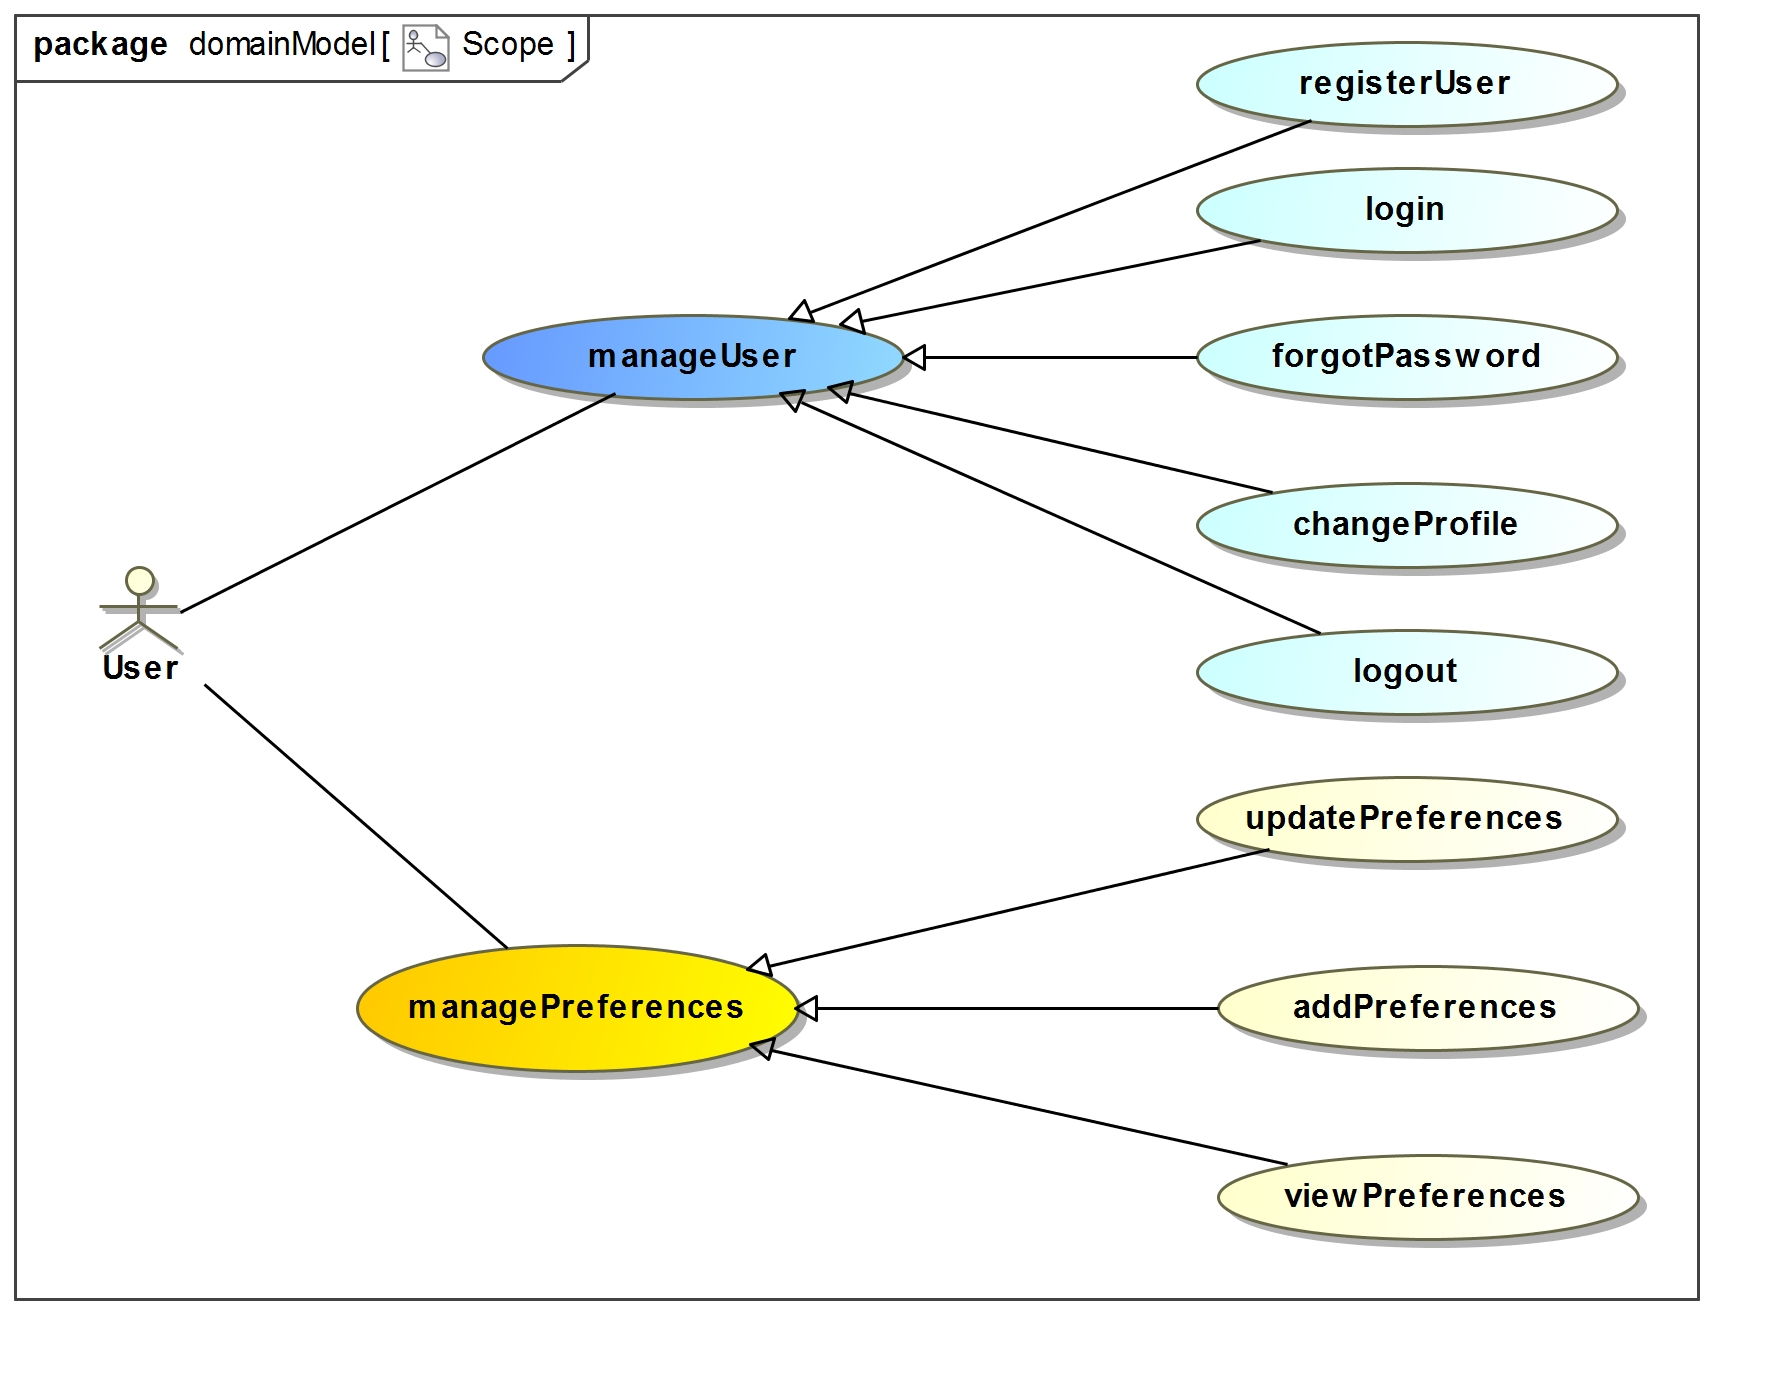
\includegraphics[width=1.0\textwidth]{../images/funcReq/UserScope.jpg}
	\caption{The scope of functionality required from the user module \label{overflow}}
\end{figure}

A user can register and login in to the system to get access to functionality such as adding,viewing and editing preferences of weather or disaster data that they would like to be at their disposal. They are also ablo to logout of the system once done.

\subsubsection{registerUser}

A user can register with the system as long as they are not already registered. Below are the service contract, activity diagram and functional requirements diagram for registerUser.

\begin{figure}[H]
	\centering
	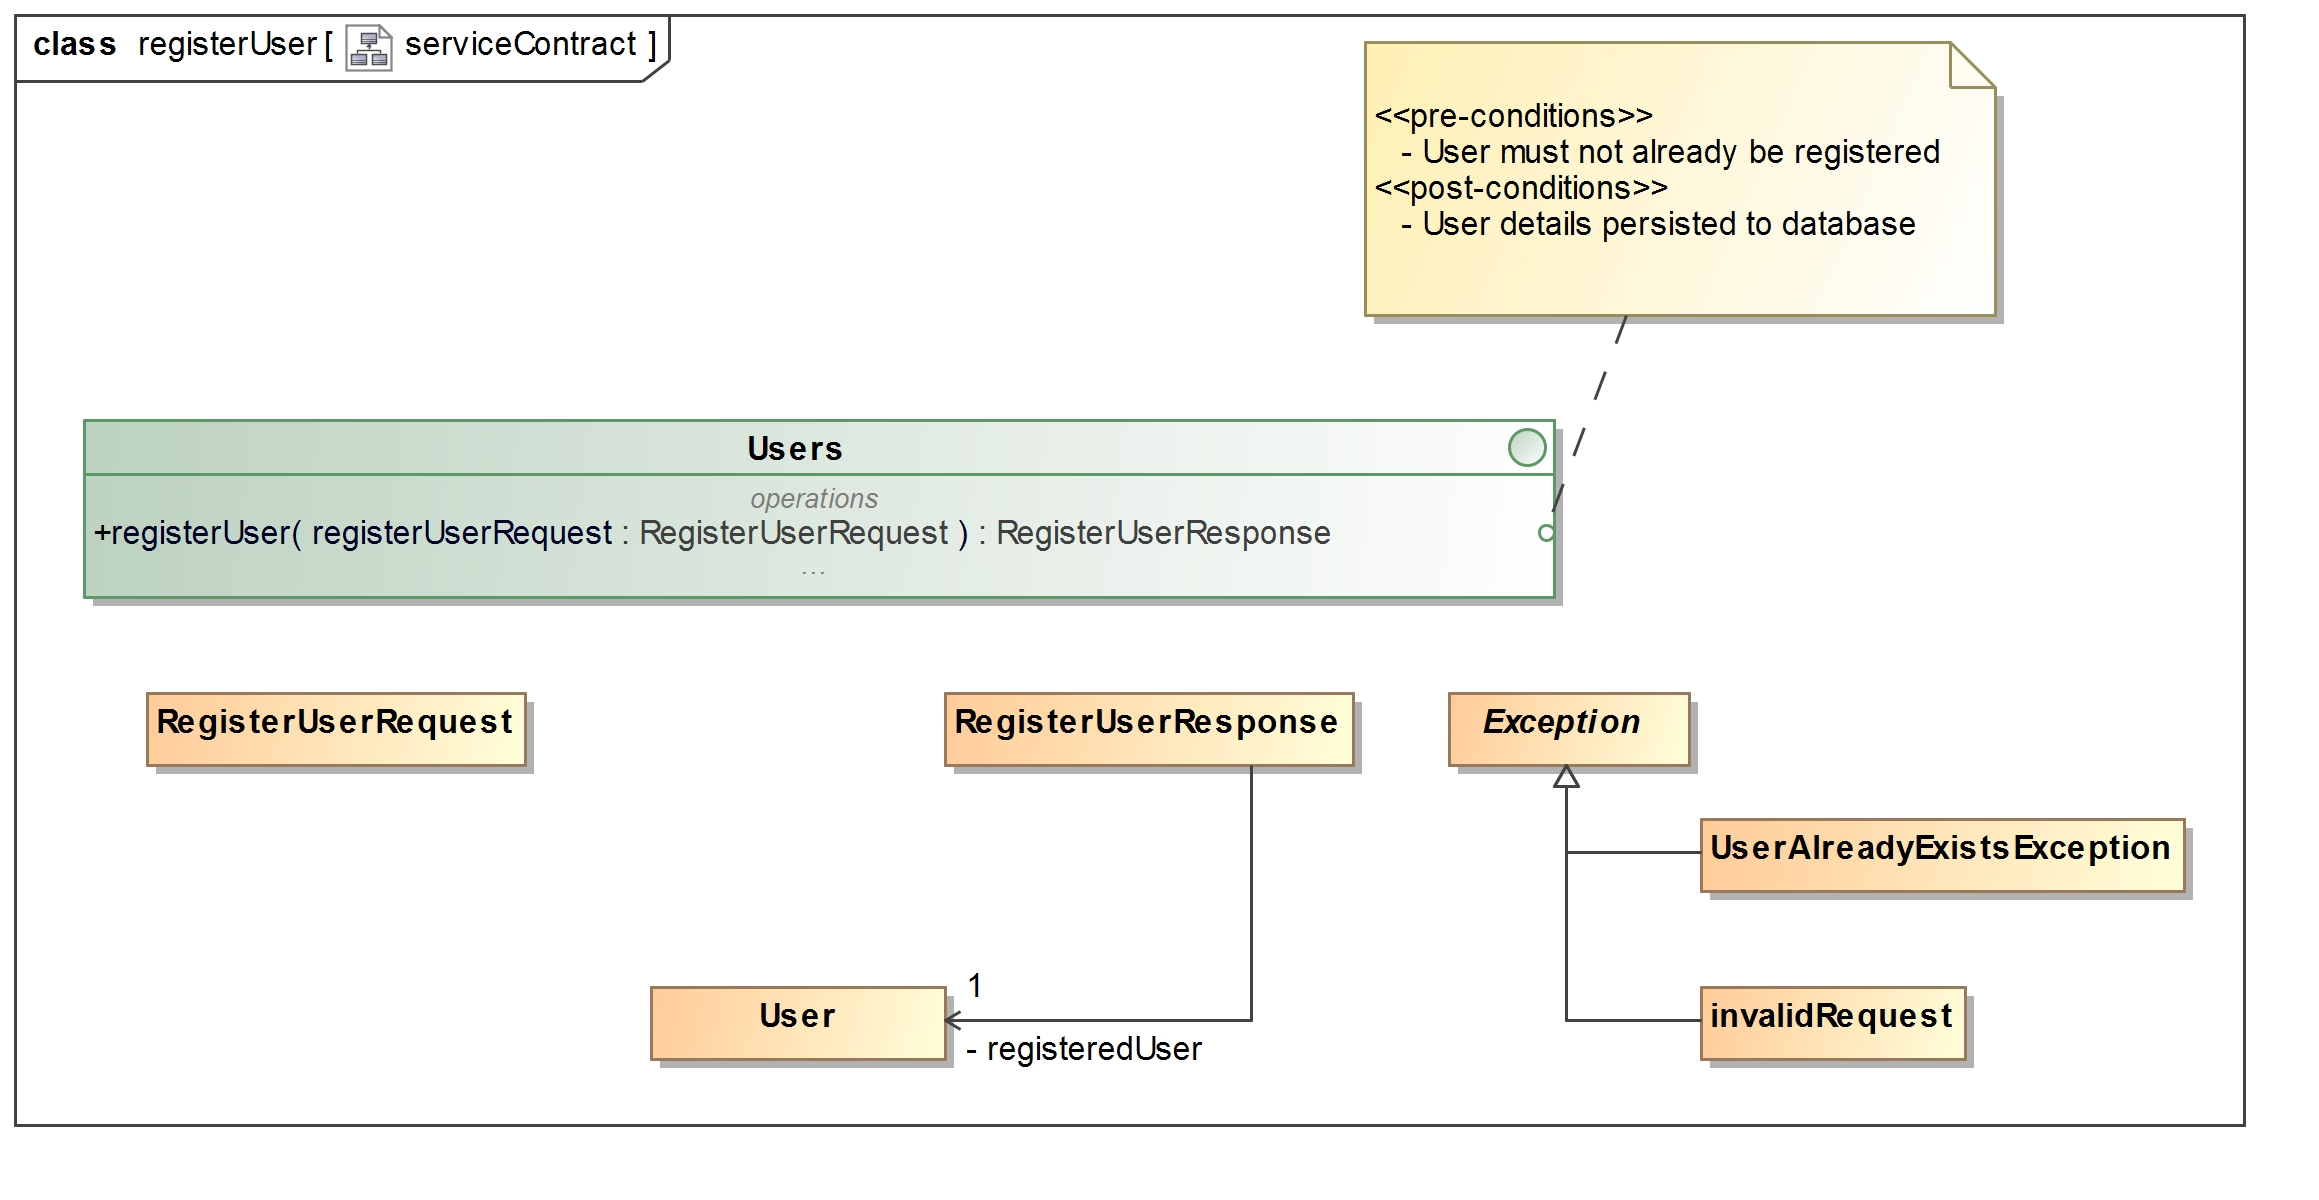
\includegraphics[scale=0.21]{../images/funcReq/registerUserServiceContract.jpg}
	\caption{The service contract for registerUser \label{overflow}}
\end{figure}

\begin{figure}[H]
	\centering
	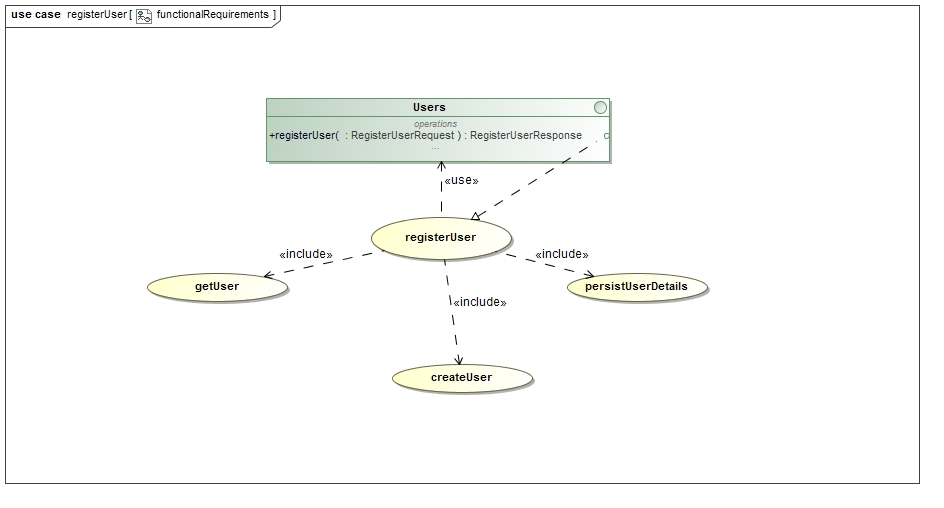
\includegraphics[width=1.1\textwidth]{../images/funcReq/registerUserFunctionalRequirements.jpg}
	\caption{The functional requirements diagram for registerUser \label{overflow}}
\end{figure}

\begin{figure}[H]
	\centering
	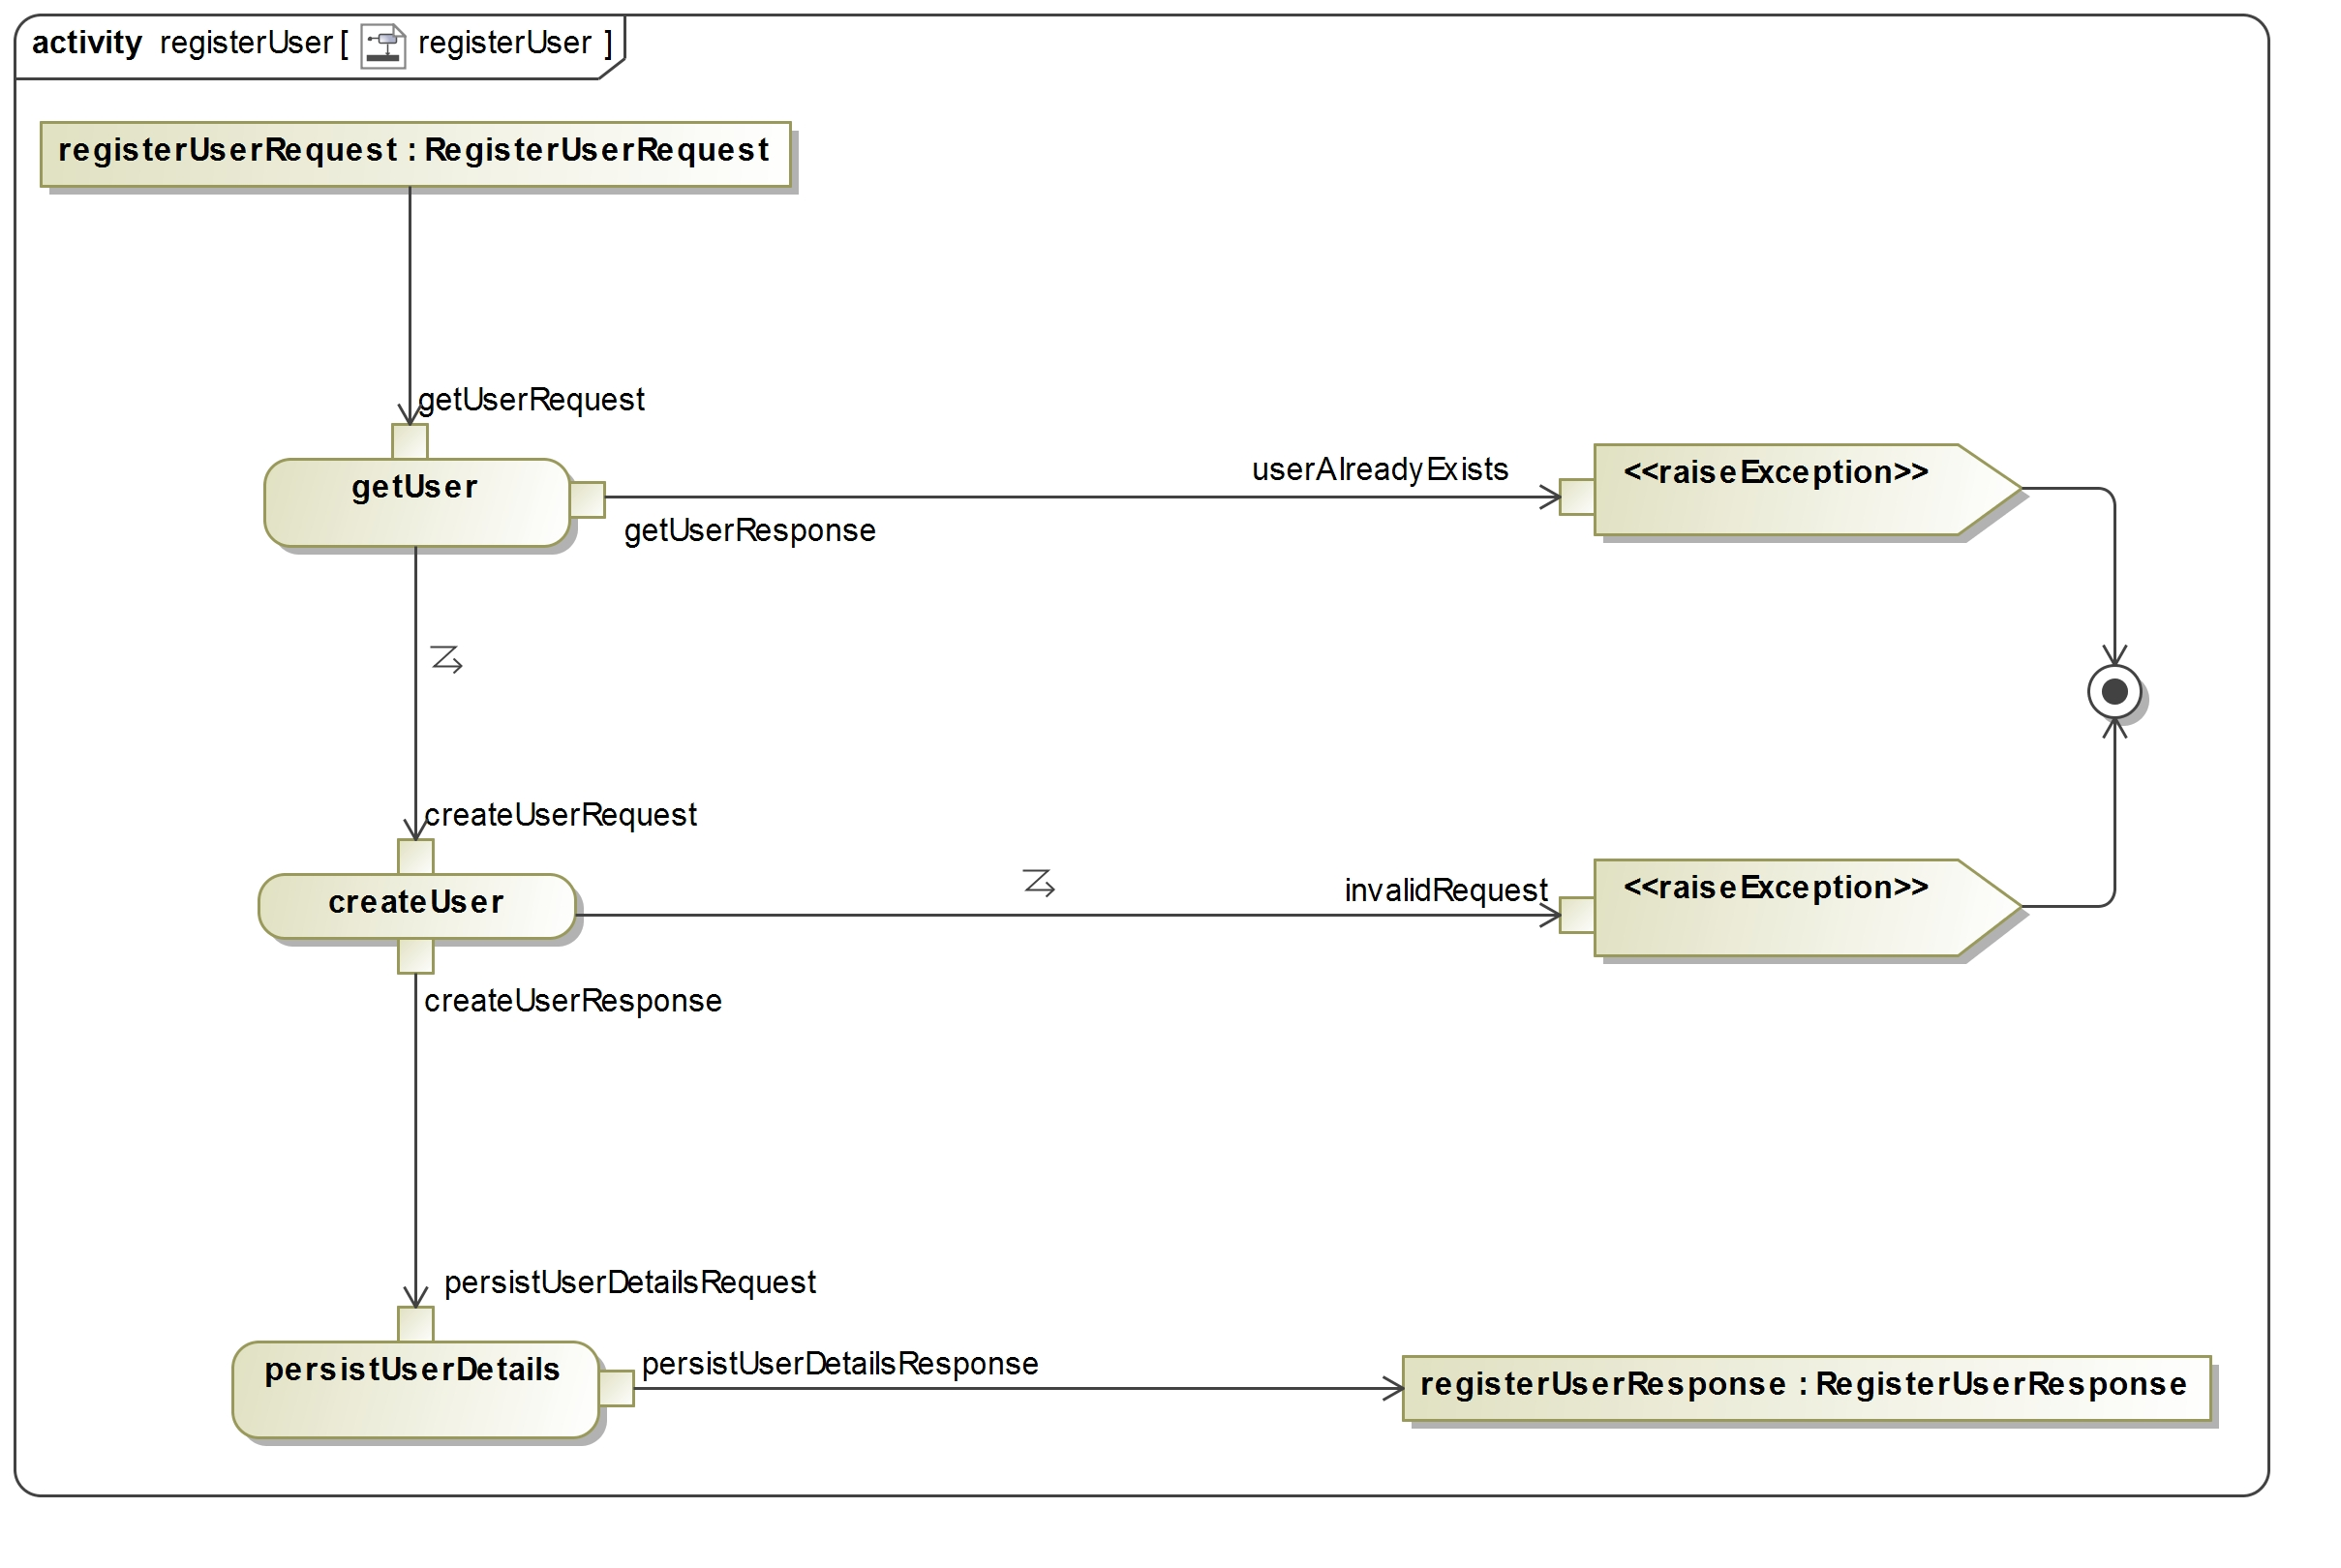
\includegraphics[scale=0.2]{../images/funcReq/registerUserActivityDiagram.jpg}
	\caption{The activity diagram for registerUser \label{overflow}}
\end{figure}

\subsubsection{login}

A registered user, given that they provide correct details to authenicate them and they are not already logged in, is able to access functionality such as adding and editing weather and disaster preferences once logged in. Below are the service contract, activity diagram and functional requirements diagram for login.

\begin{figure}[H]
	\centering
	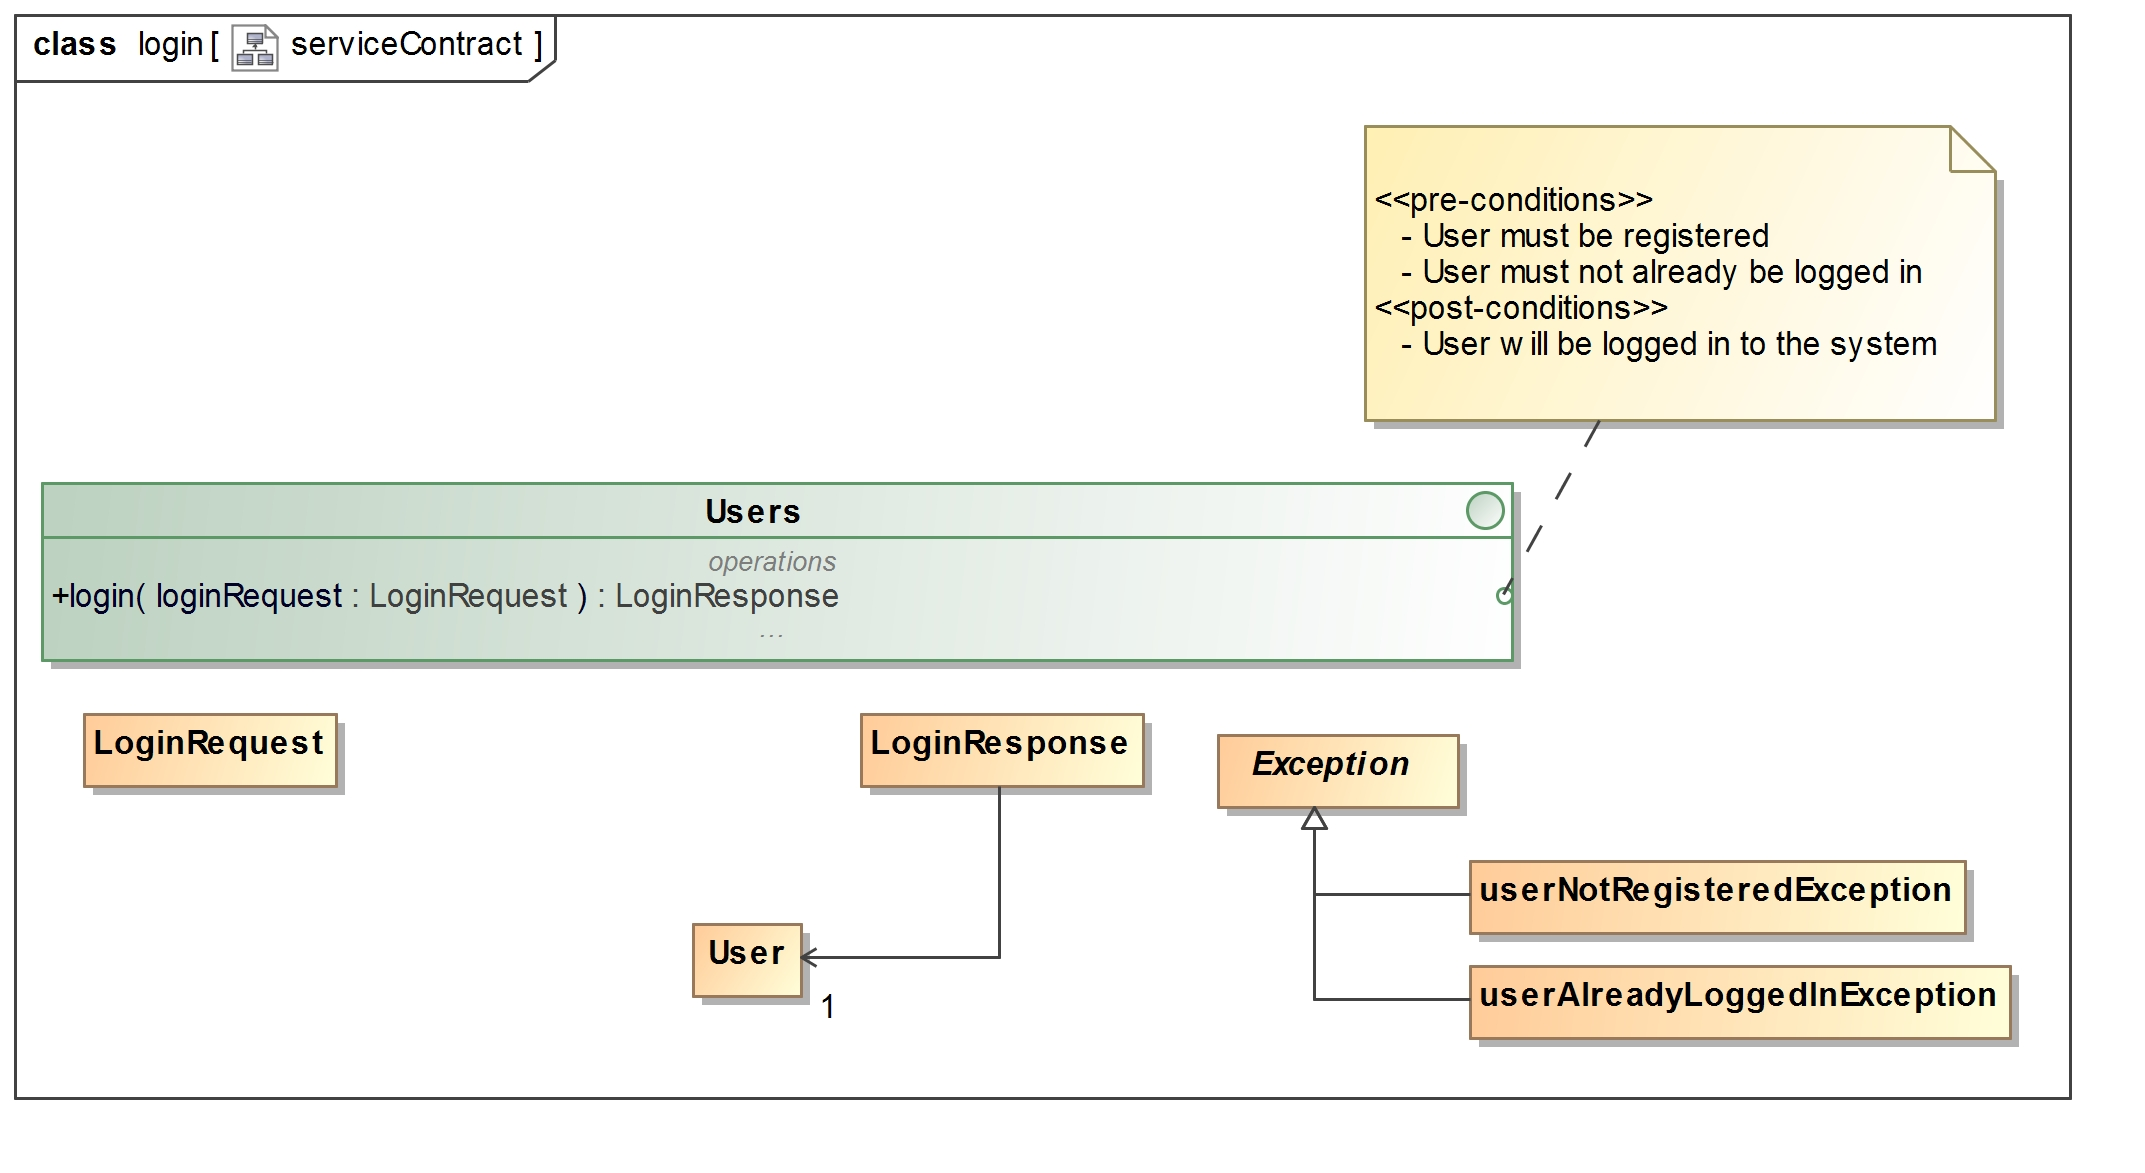
\includegraphics[width=1.2\textwidth]{../images/funcReq/loginServiceContract.jpg}
	\caption{The service contract for login \label{overflow}}
\end{figure}

\begin{figure}[H]
	\centering
	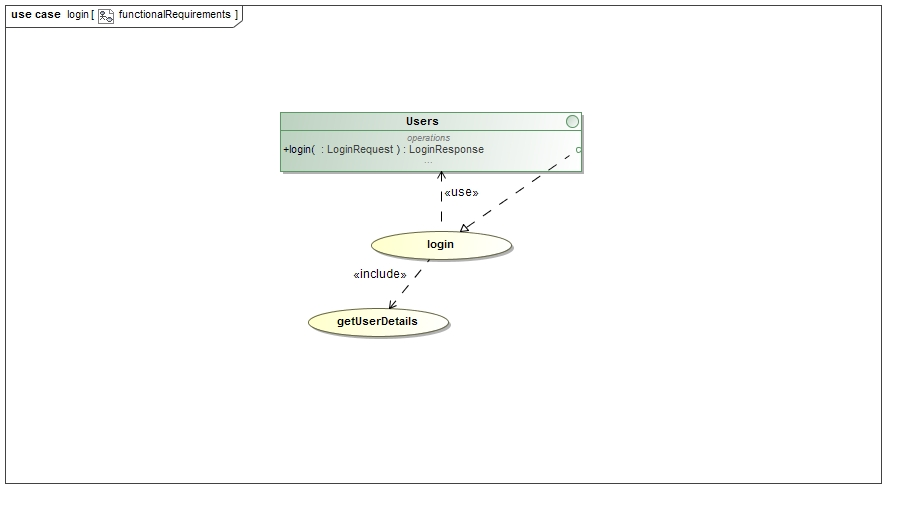
\includegraphics[width=1.1\textwidth]{../images/funcReq/loginFunctionalRequirements.jpg}
	\caption{The functional requirements diagram for login \label{overflow}}
\end{figure}

\begin{figure}[H]
	\centering
	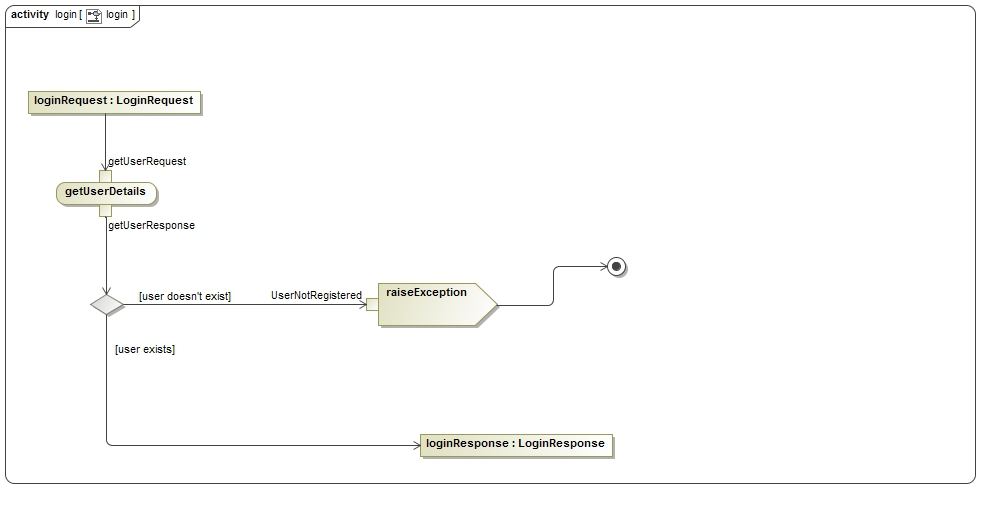
\includegraphics[width=1.1\textwidth]{../images/funcReq/loginActivityDiagram.jpg}
	\caption{The activity diagram for login \label{overflow}}
\end{figure}

\subsubsection{forgotPassword}

A user who has forgotten their password is able to have it sent to them via email as long as they provide a working email address that is registered with the system.  Below are the service contract, activity diagram and functional requirements diagram for forgotPassword.

\begin{figure}[H]
	\centering
	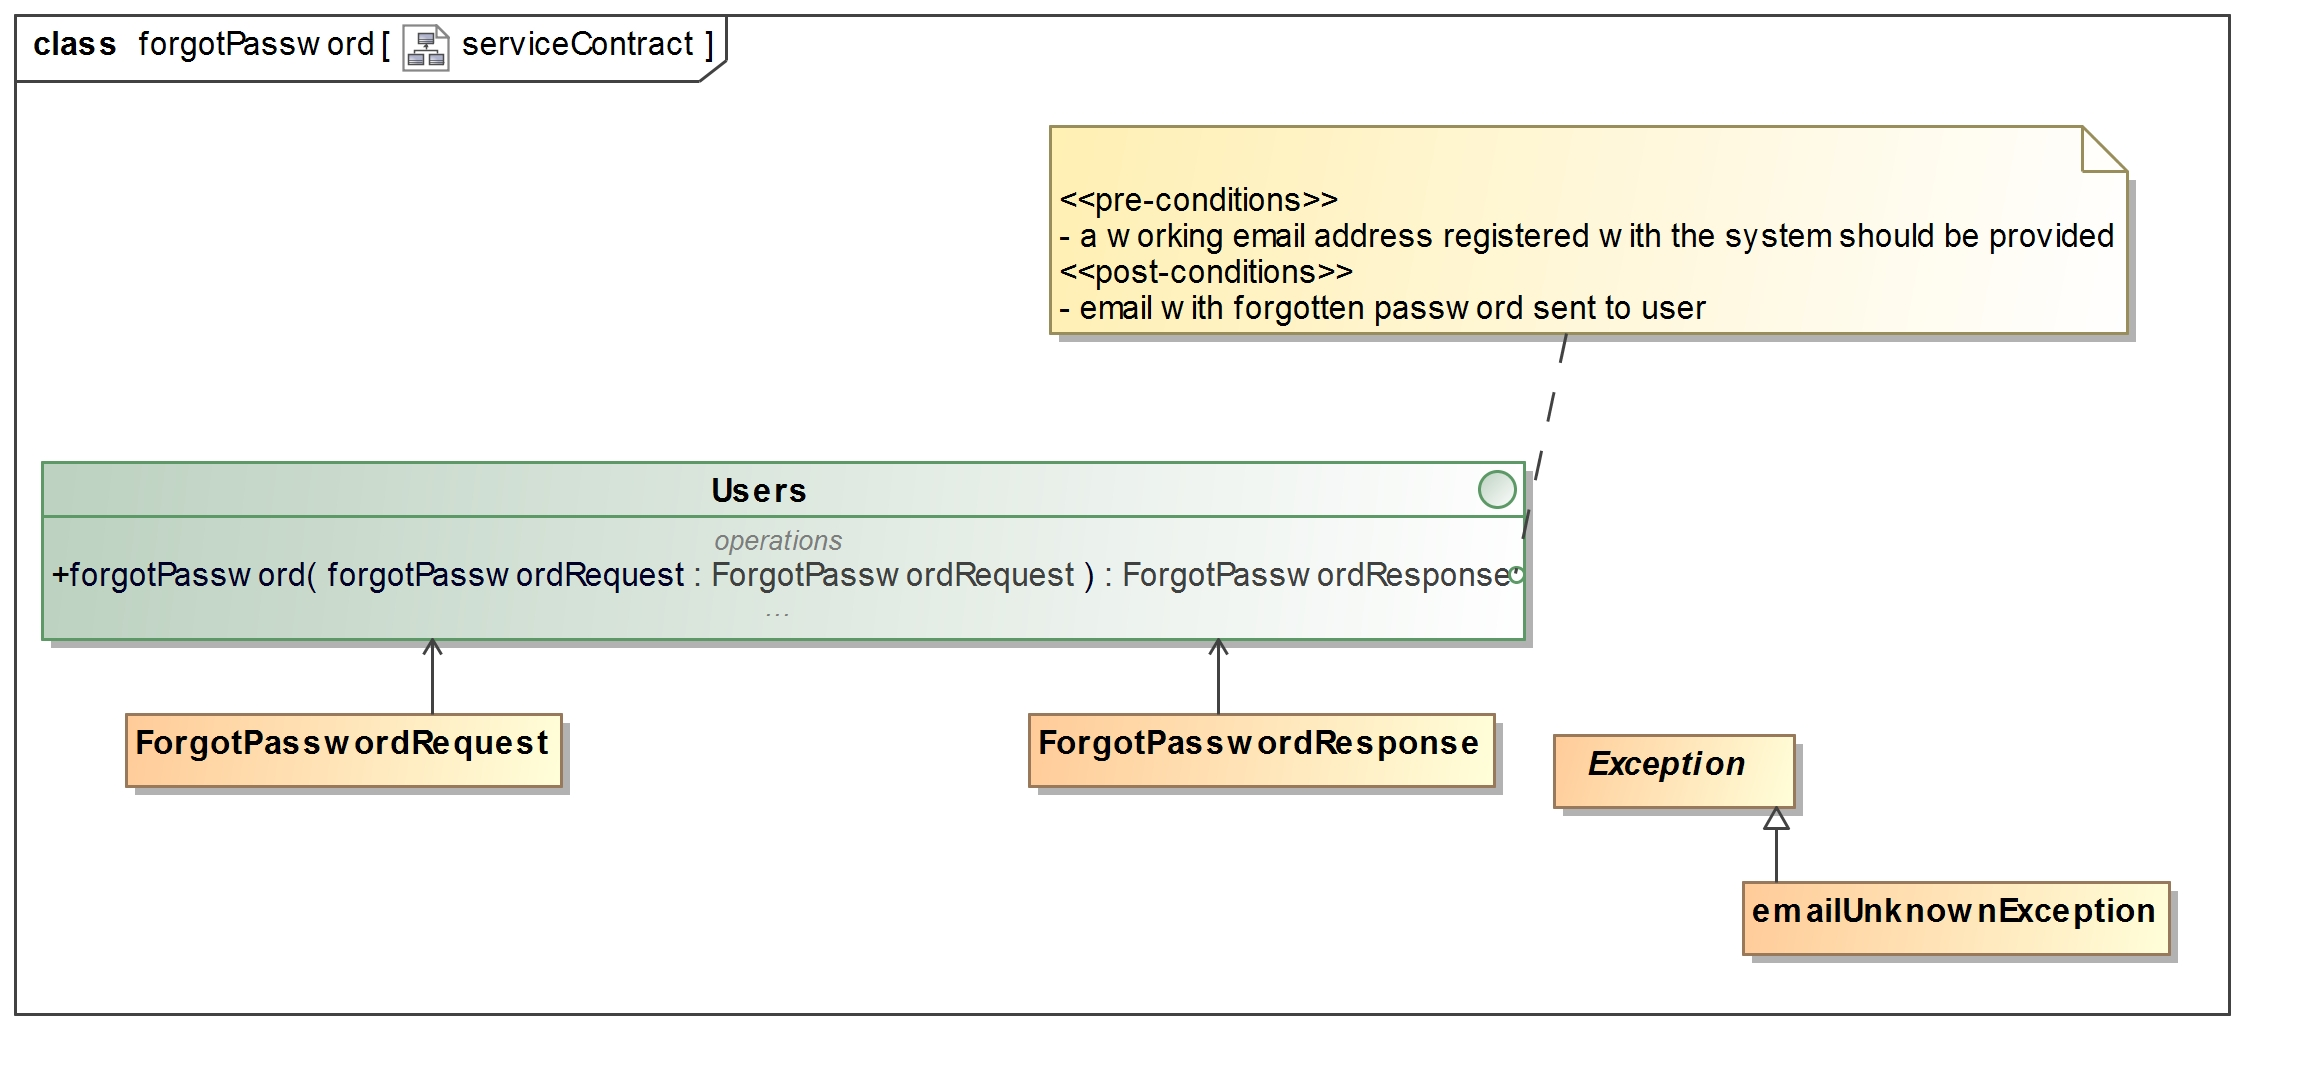
\includegraphics[scale=0.21]{../images/funcReq/forgotPasswordServiceContract.jpg}
	\caption{The service contract for forgotPassword \label{overflow}}
\end{figure}

\begin{figure}[H]
	\centering
	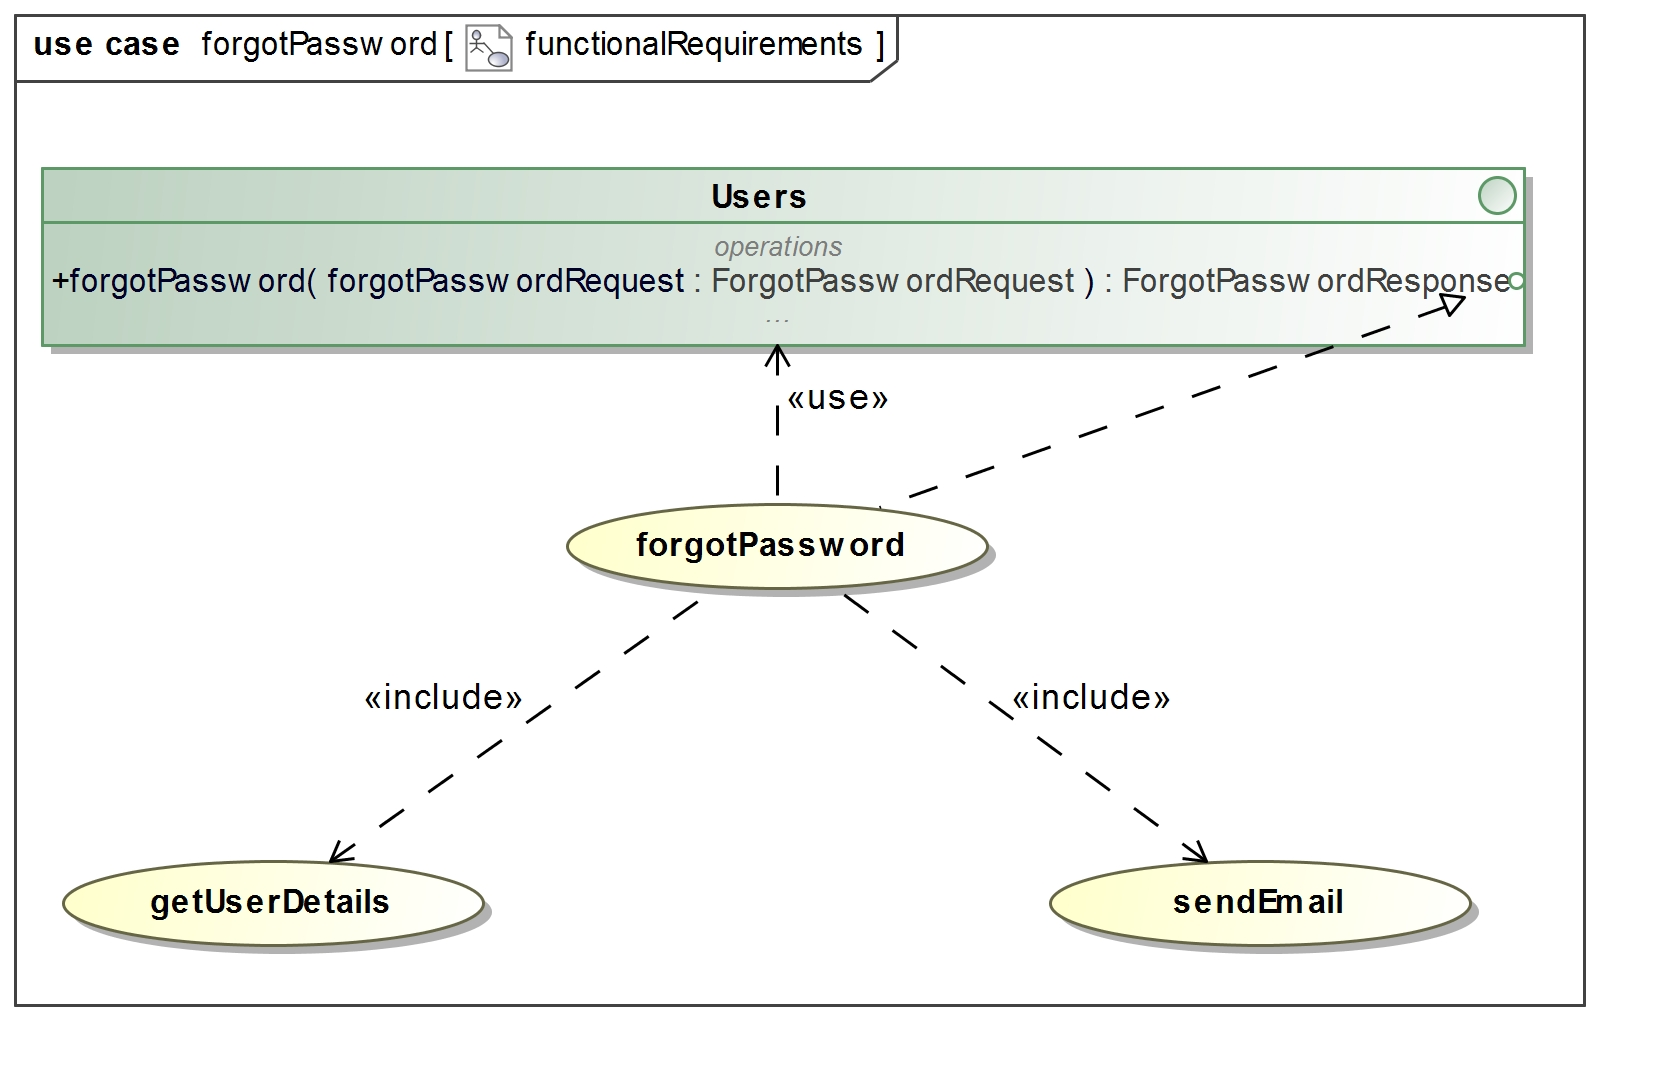
\includegraphics[width=1.1\textwidth]{../images/funcReq/forgotPasswordFunctionalRequirements.jpg}
	\caption{The functional requirements diagram for forgotPassword \label{overflow}}
\end{figure}

\begin{figure}[H]
	\centering
	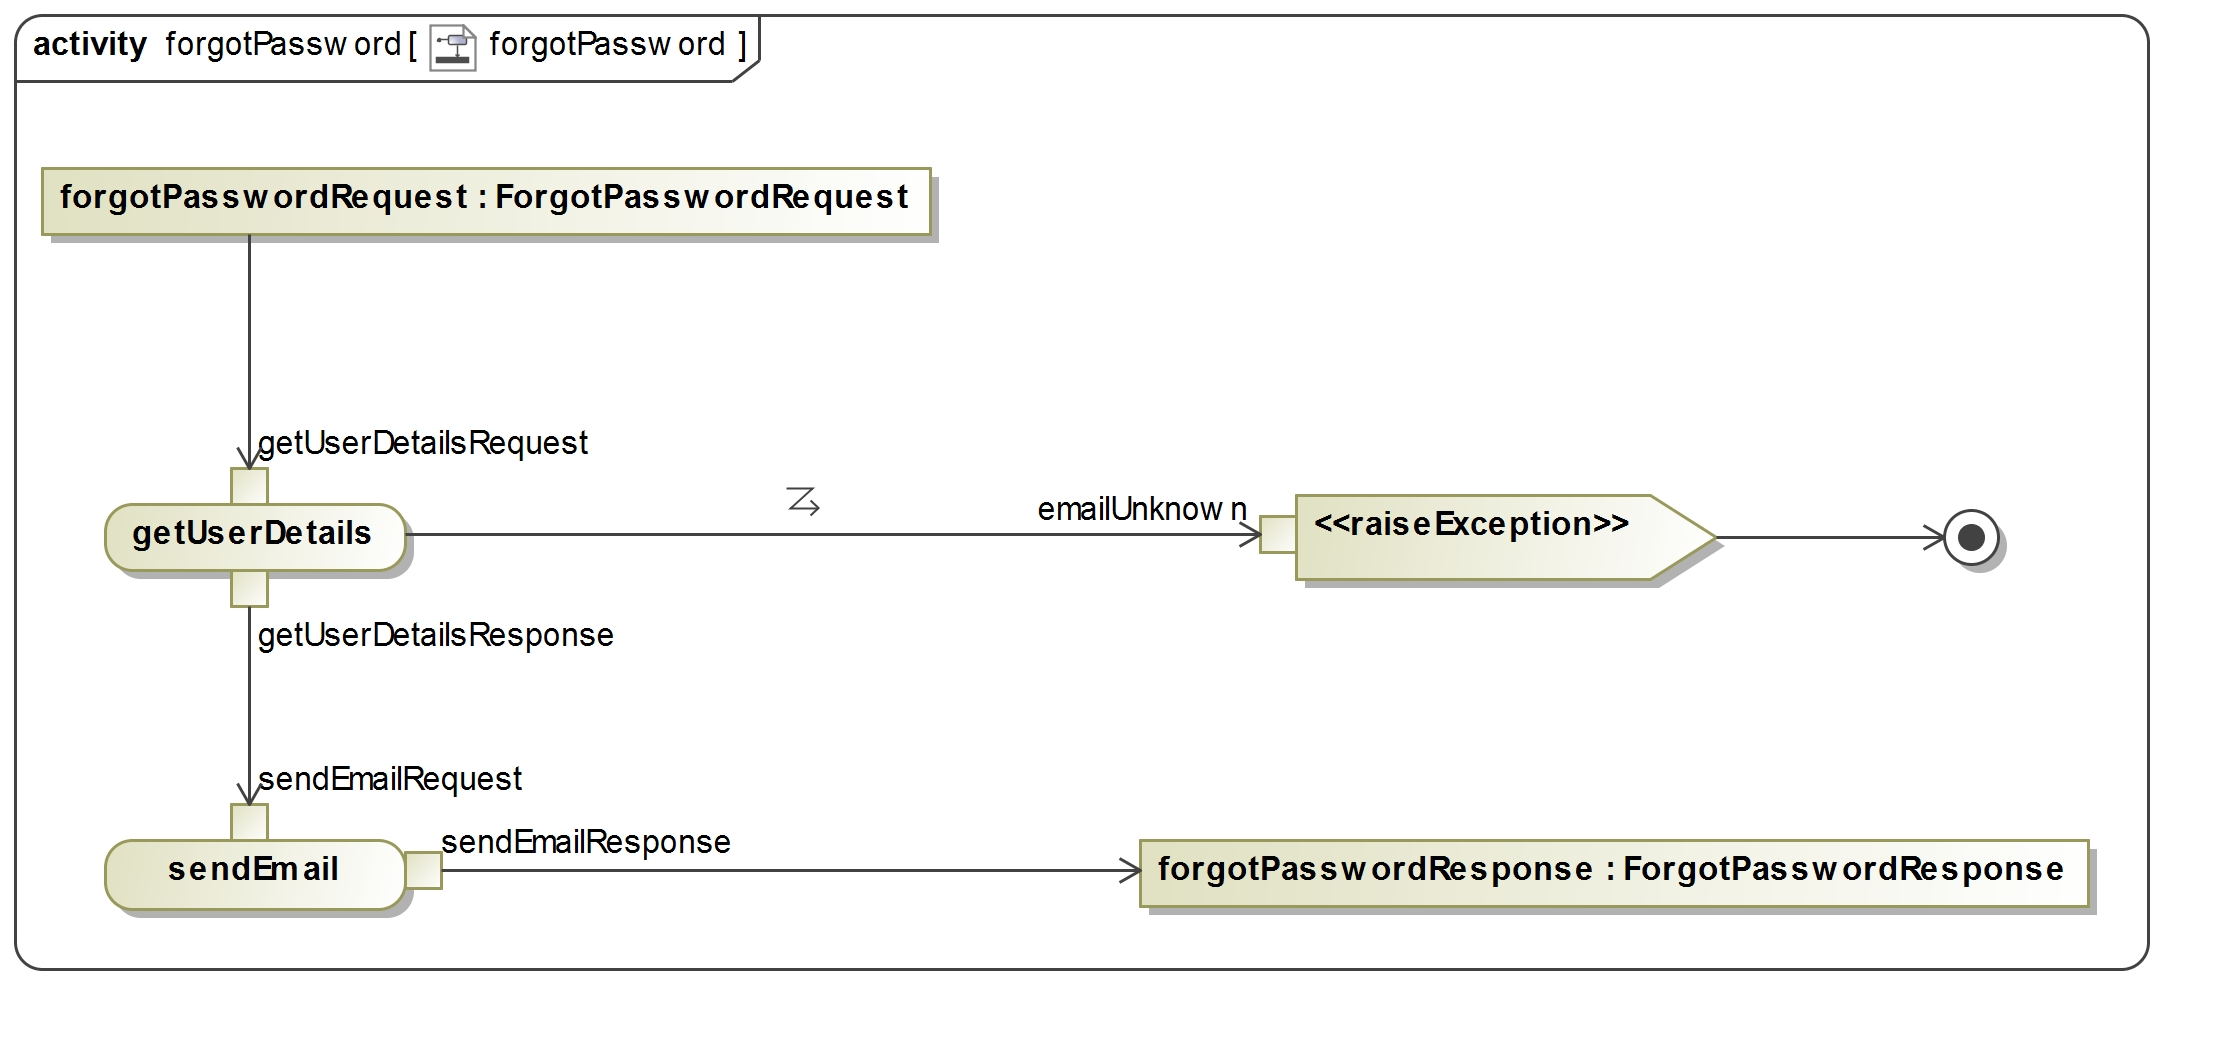
\includegraphics[scale=0.22]{../images/funcReq/forgotPasswordActivityDiagram.jpg}
	\caption{The activity diagram for forgotPassword \label{overflow}}
\end{figure}

\subsubsection{changeProfile}

A user, given that they are logged in, is able to change their user profile. Below are the service contract, activity diagram and functional requirements diagram for changeProfile.

\begin{figure}[H]
	\centering
	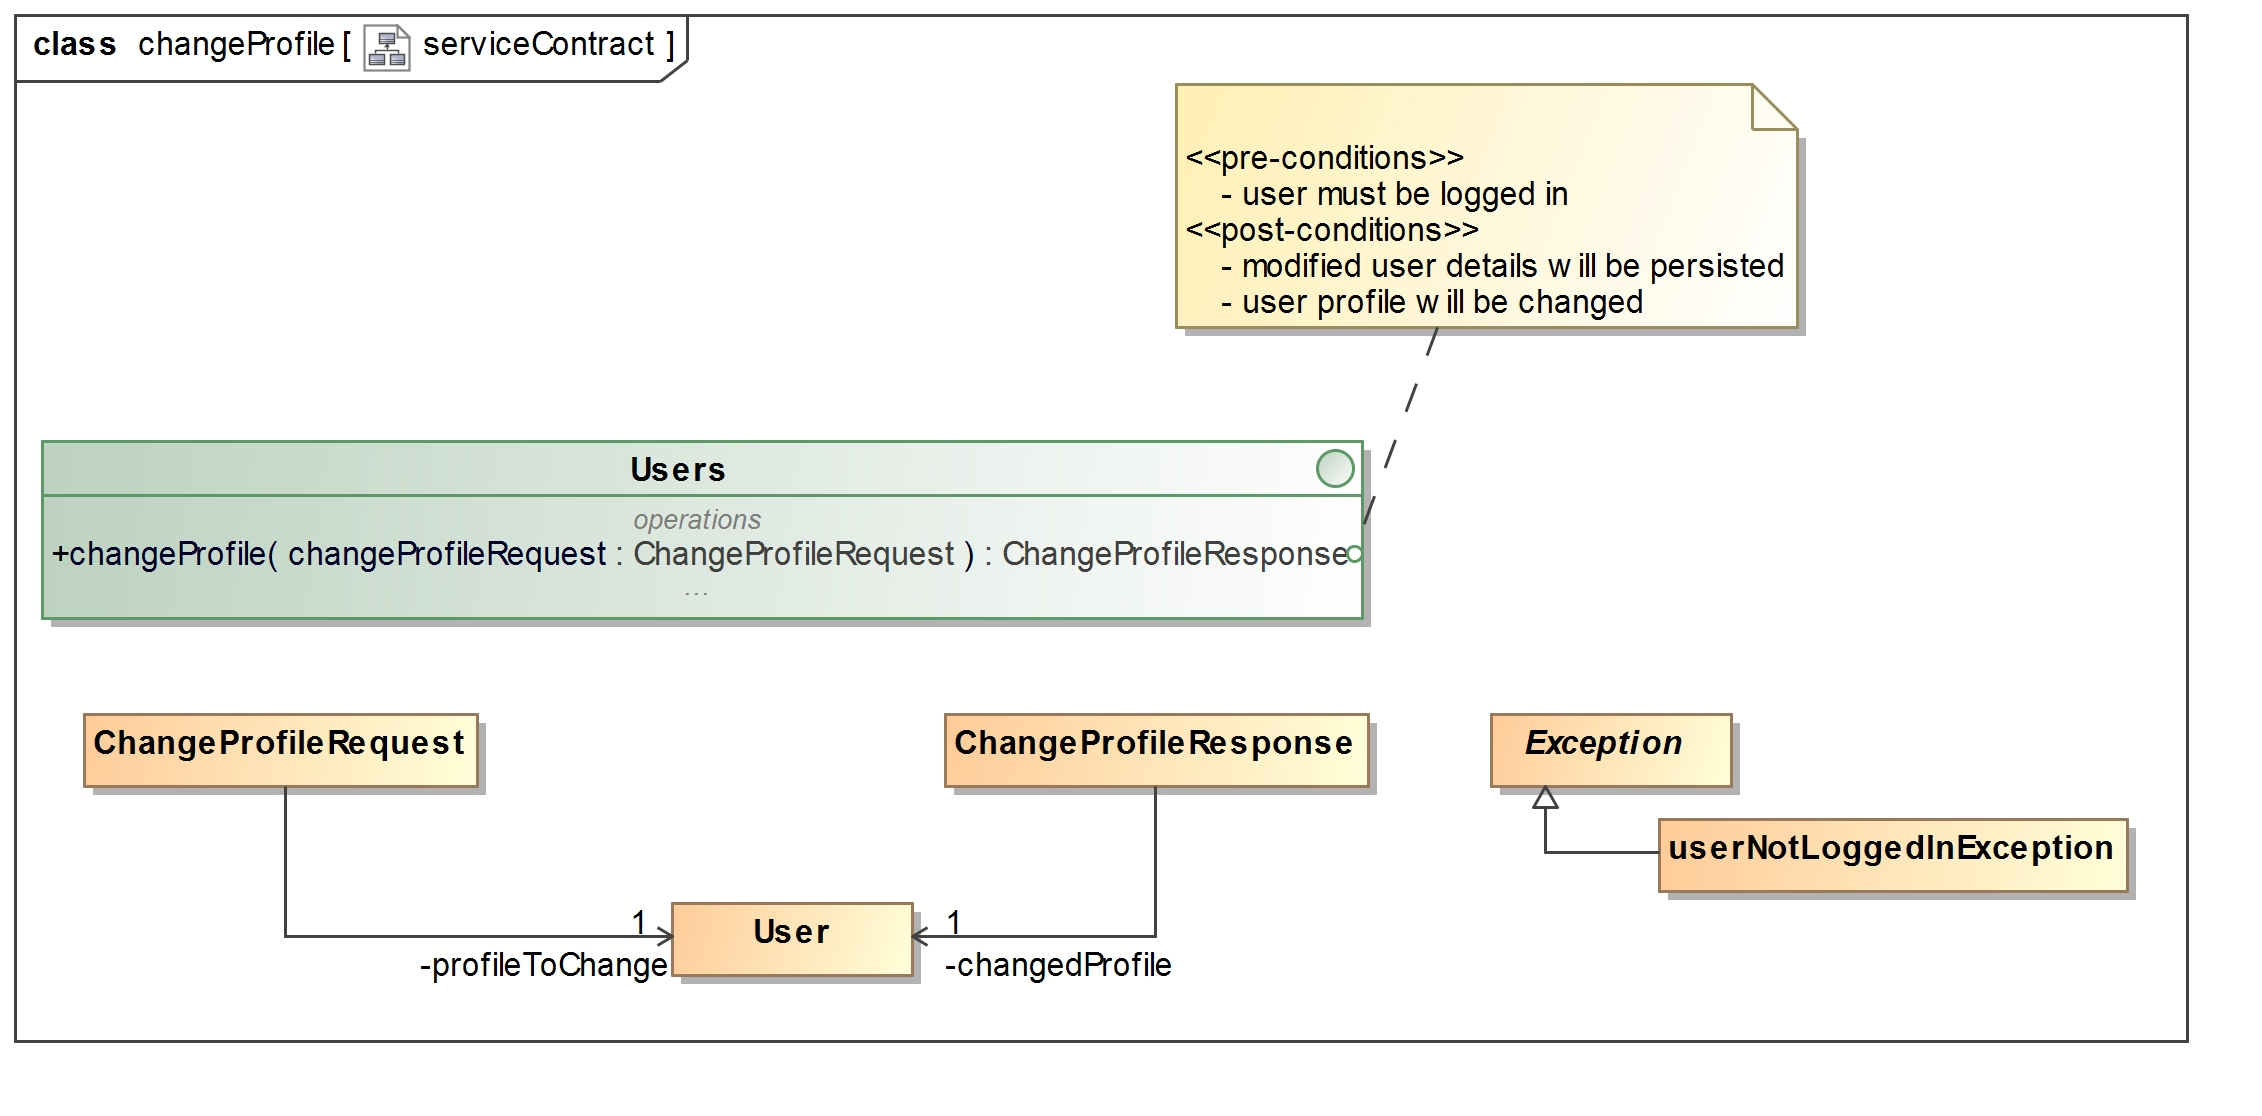
\includegraphics[scale=0.22]{../images/funcReq/changeProfileServiceContract.jpg}
	\caption{The service contract for changeProfile \label{overflow}}
\end{figure}

\begin{figure}[H]
	\centering
	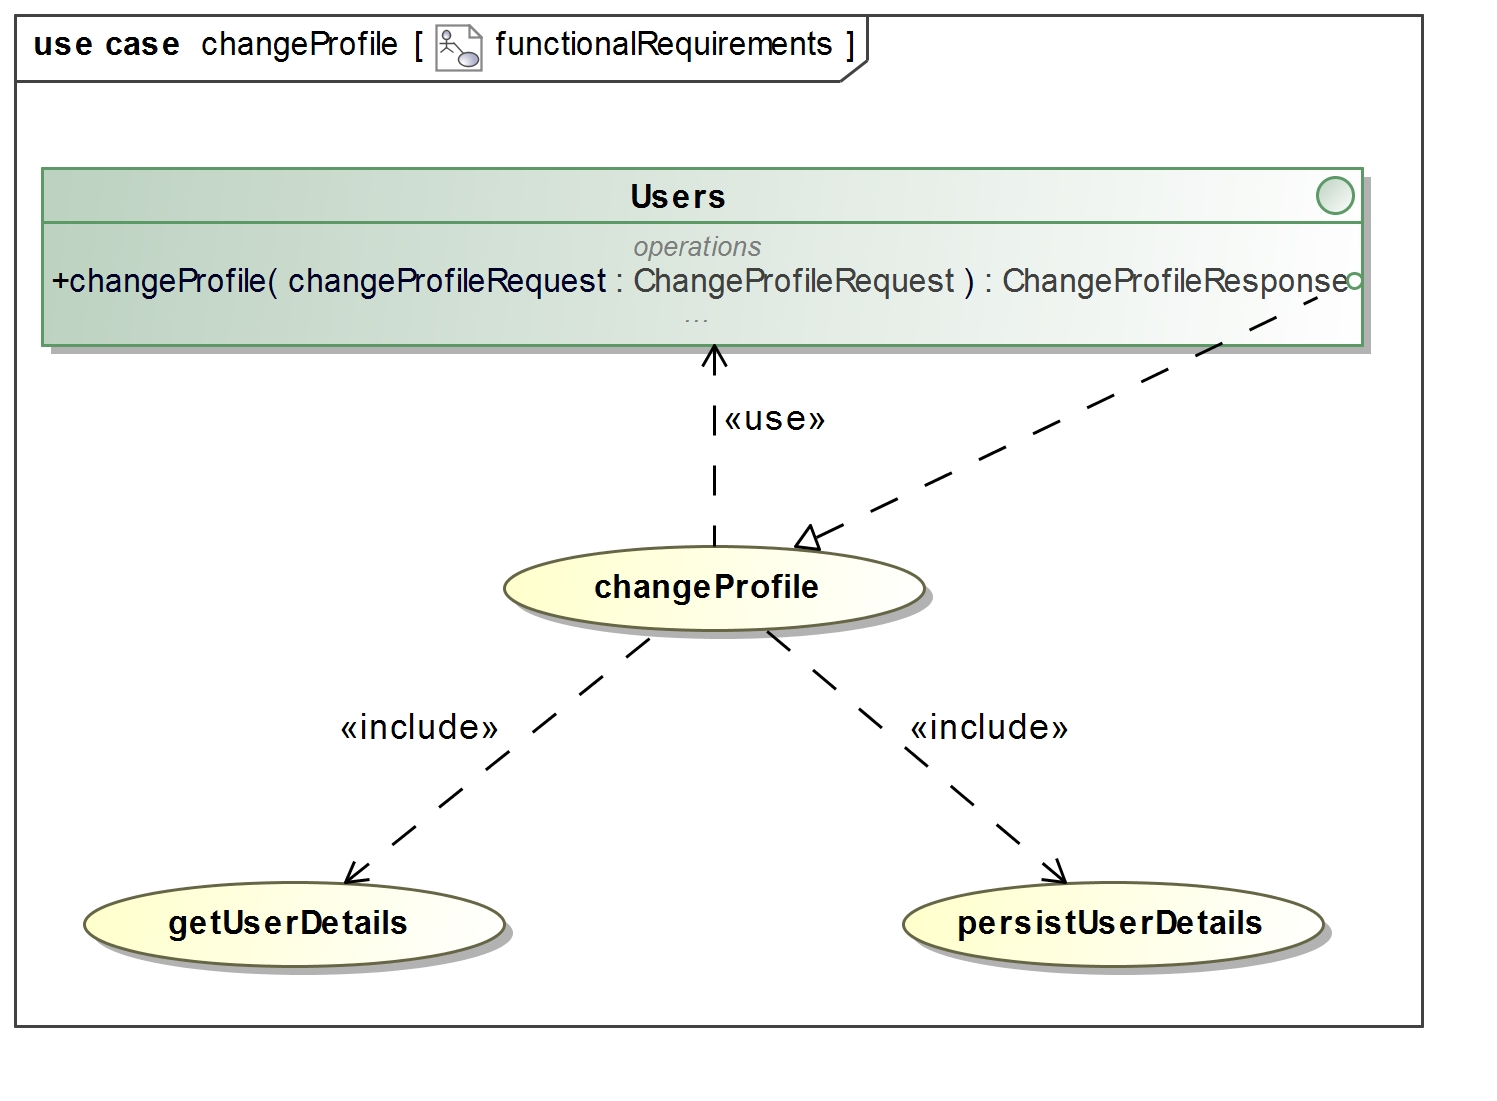
\includegraphics[width=1.1\textwidth]{../images/funcReq/changeProfileFunctionalRequirements.jpg}
	\caption{The functional requirements diagram for changeProfile \label{overflow}}
\end{figure}

\begin{figure}[H]
	\centering
	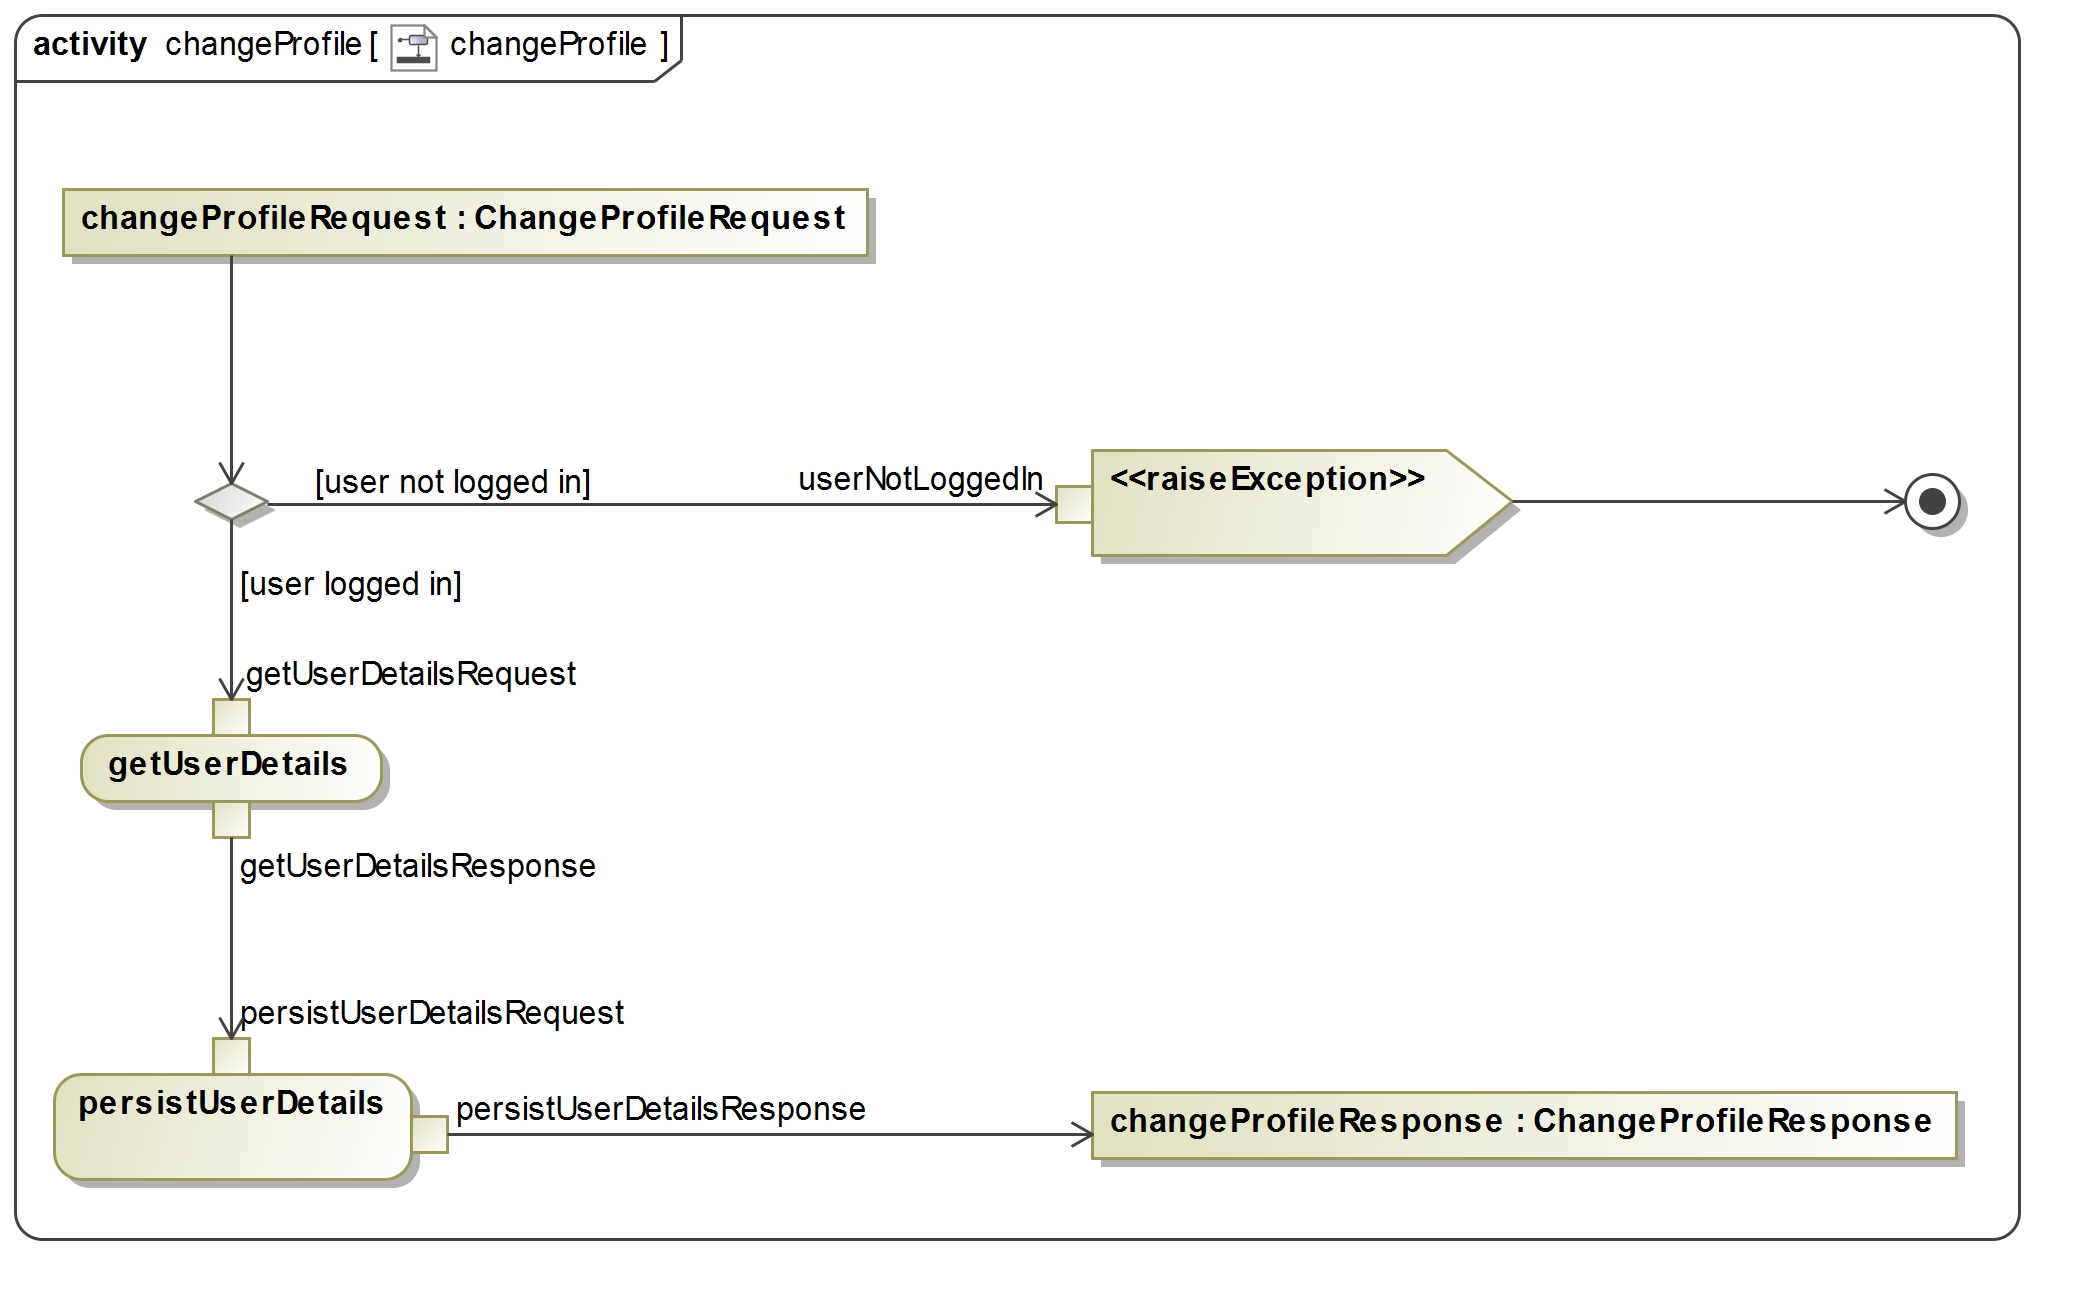
\includegraphics[scale=0.22]{../images/funcReq/changeProfileActivityDiagram.jpg}
	\caption{The activity diagram for changeProfile \label{overflow}}
\end{figure}

\subsubsection{logout}

A user, given that they are logged in to the system, is able to logout of the system once done. Below are the service contract, activity diagram and functional requirements diagram for logout.

\begin{figure}[H]
	\centering
	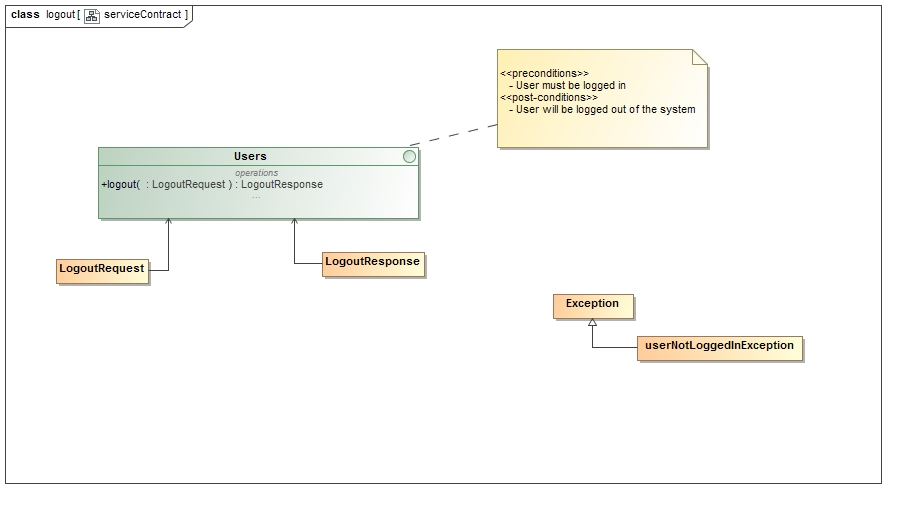
\includegraphics[width=1.2\textwidth]{../images/funcReq/logoutServiceContract.jpg}
	\caption{The service contract for logout \label{overflow}}
\end{figure}

\begin{figure}[H]
	\centering
	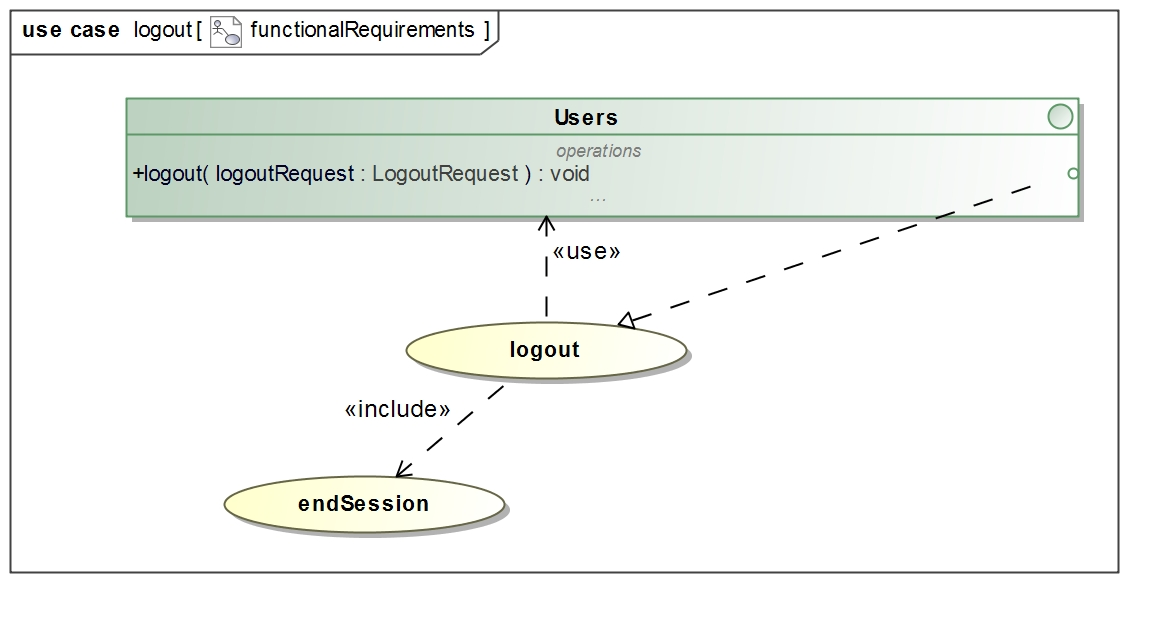
\includegraphics[width=1.1\textwidth]{../images/funcReq/logoutFunctionalRequirements.jpg}
	\caption{The functional requirements diagram for logout \label{overflow}}
\end{figure}

\begin{figure}[H]
	\centering
	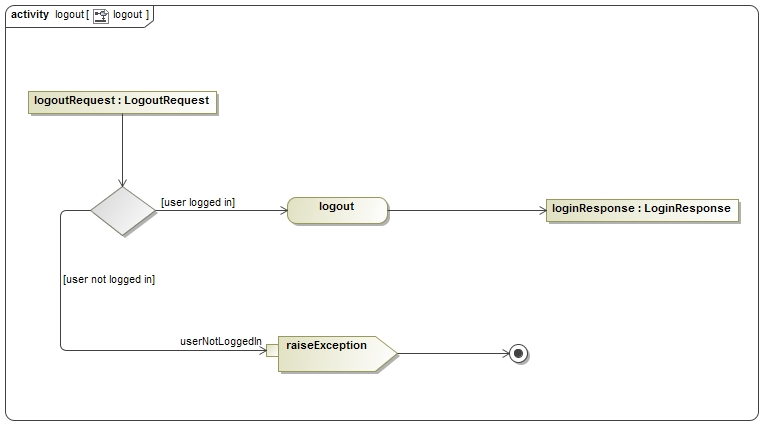
\includegraphics[scale=0.22]{../images/funcReq/logoutActivityDiagram.jpg}
	\caption{The activity diagram for logout \label{overflow}}
\end{figure}

\subsubsection{addPreferences}

A user, given that they are logged into the system, is able to add their weather and/or disaster data preferences as long as the user has specified the preference details correctly and those preference details do not already exist for the user. Below are the service contract, activity diagram and functional requirements diagram for addPreferences.

\begin{figure}[H]
	\centering
	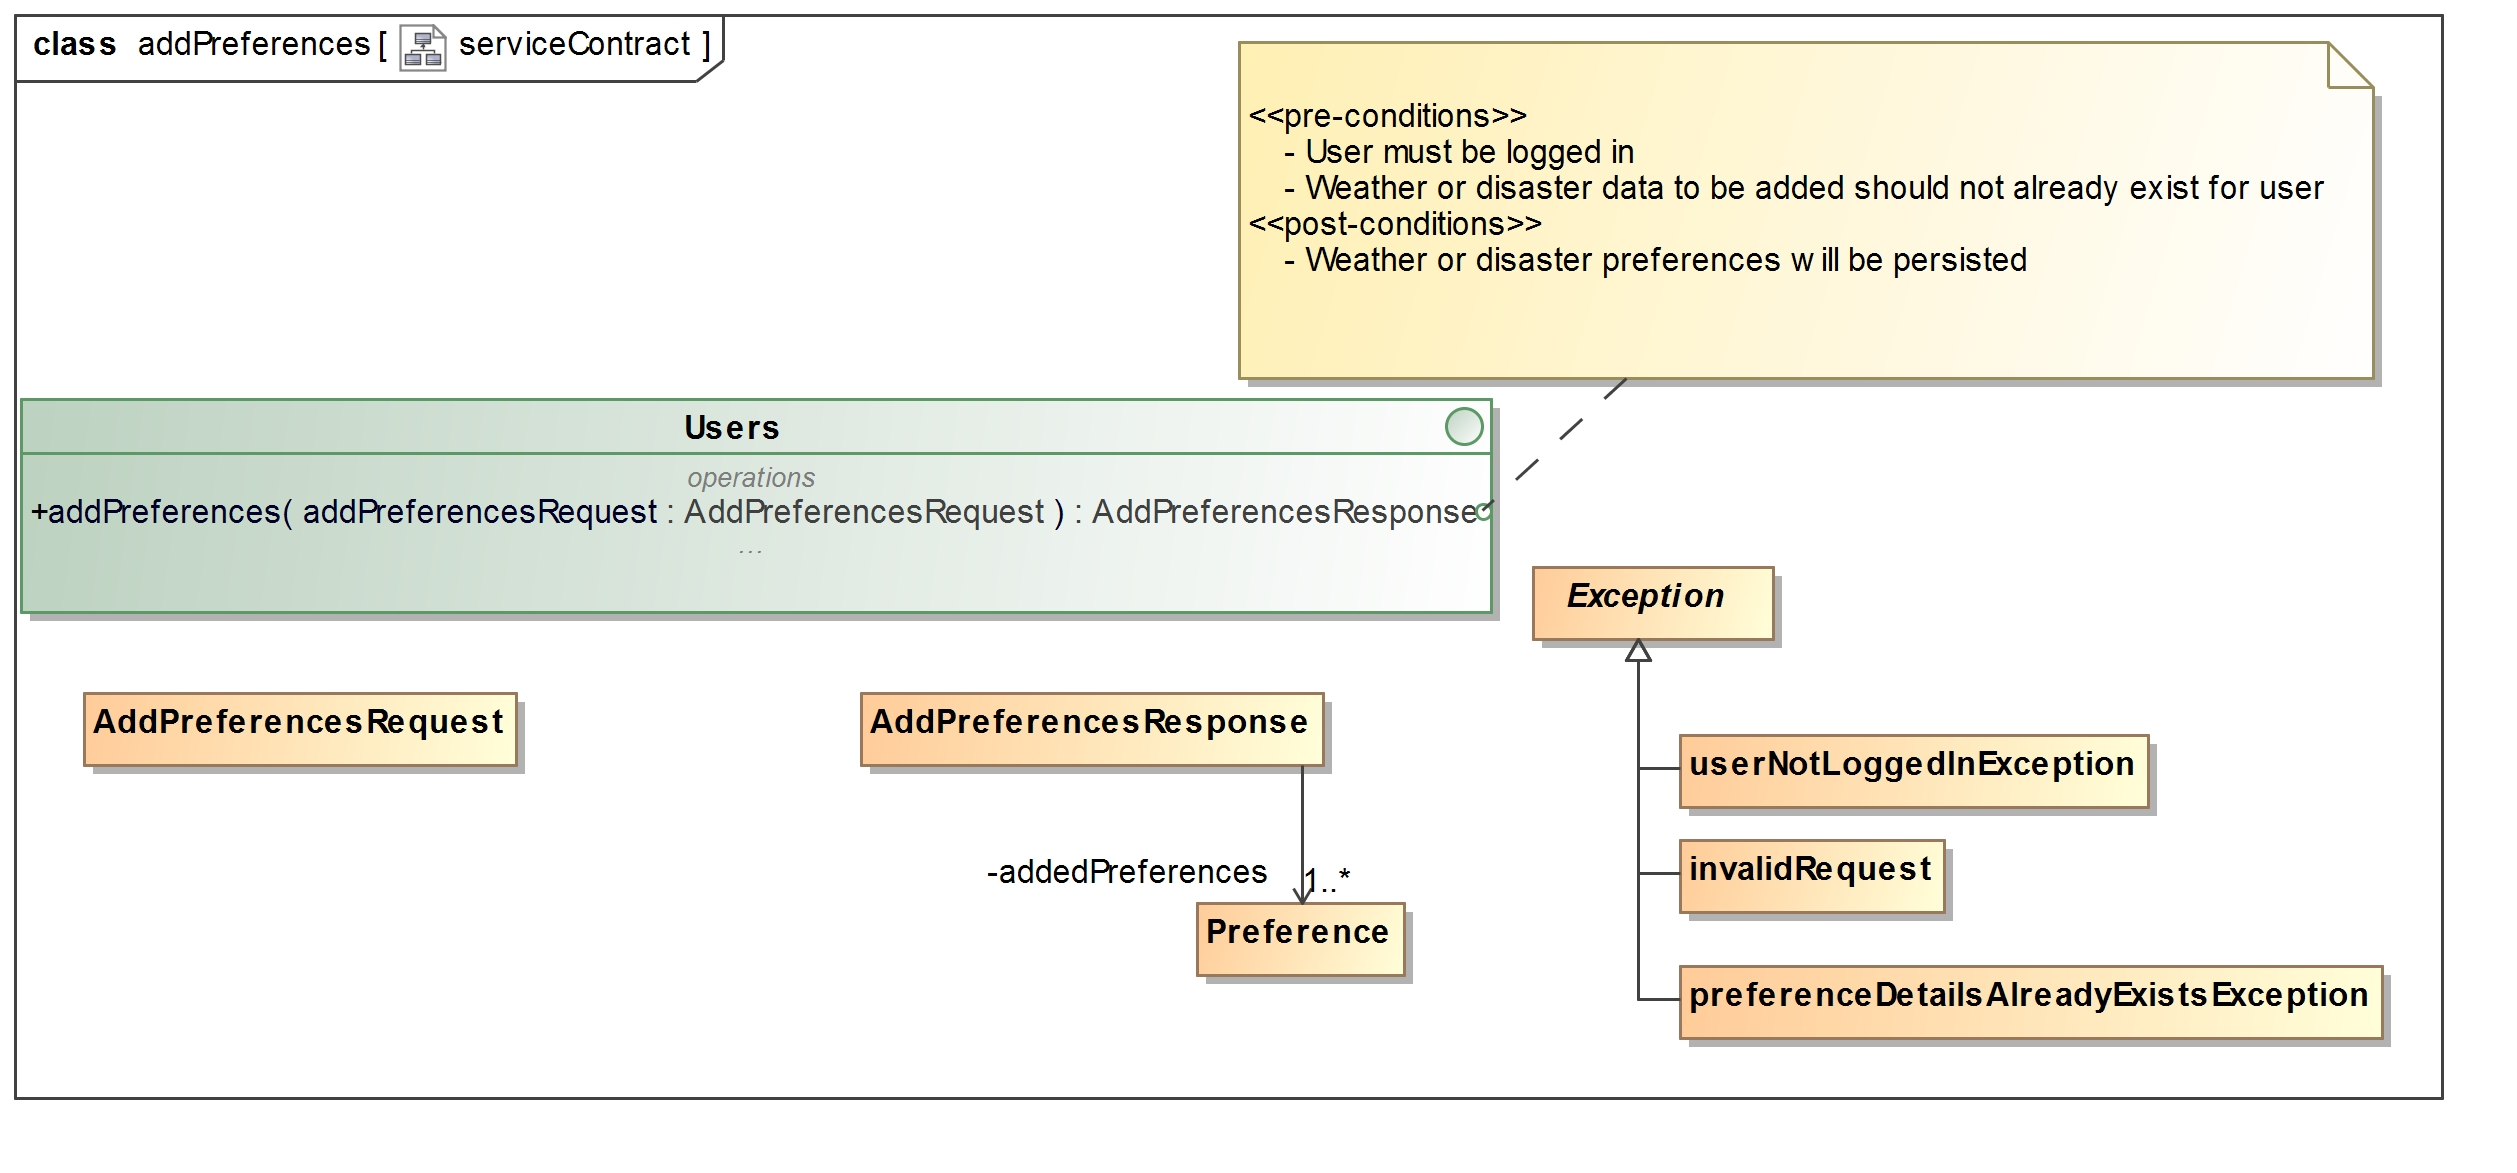
\includegraphics[scale=0.2]{../images/funcReq/addPreferencesServiceContract.jpg}
	\caption{The service contract for addPreferences \label{overflow}}
\end{figure}

\begin{figure}[H]
	\centering
	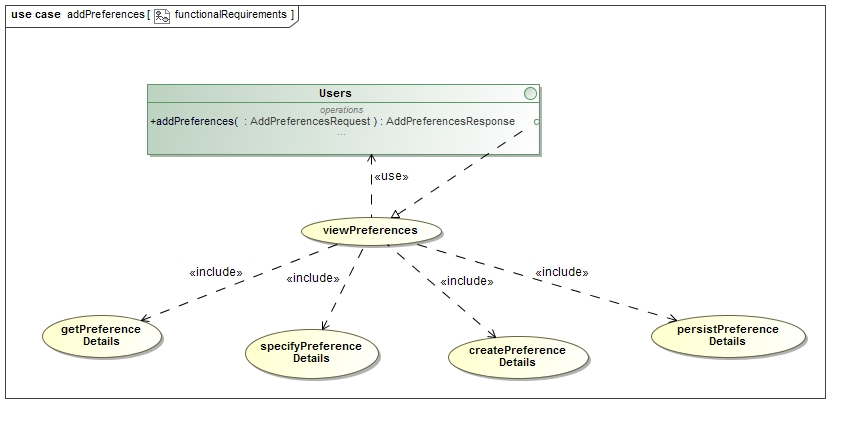
\includegraphics[scale=0.25]{../images/funcReq/addPreferencesFunctionalRequirements.jpg}
	\caption{The functional requirements diagram for addPreferences \label{overflow}}
\end{figure}

\begin{figure}[H]
	\centering
	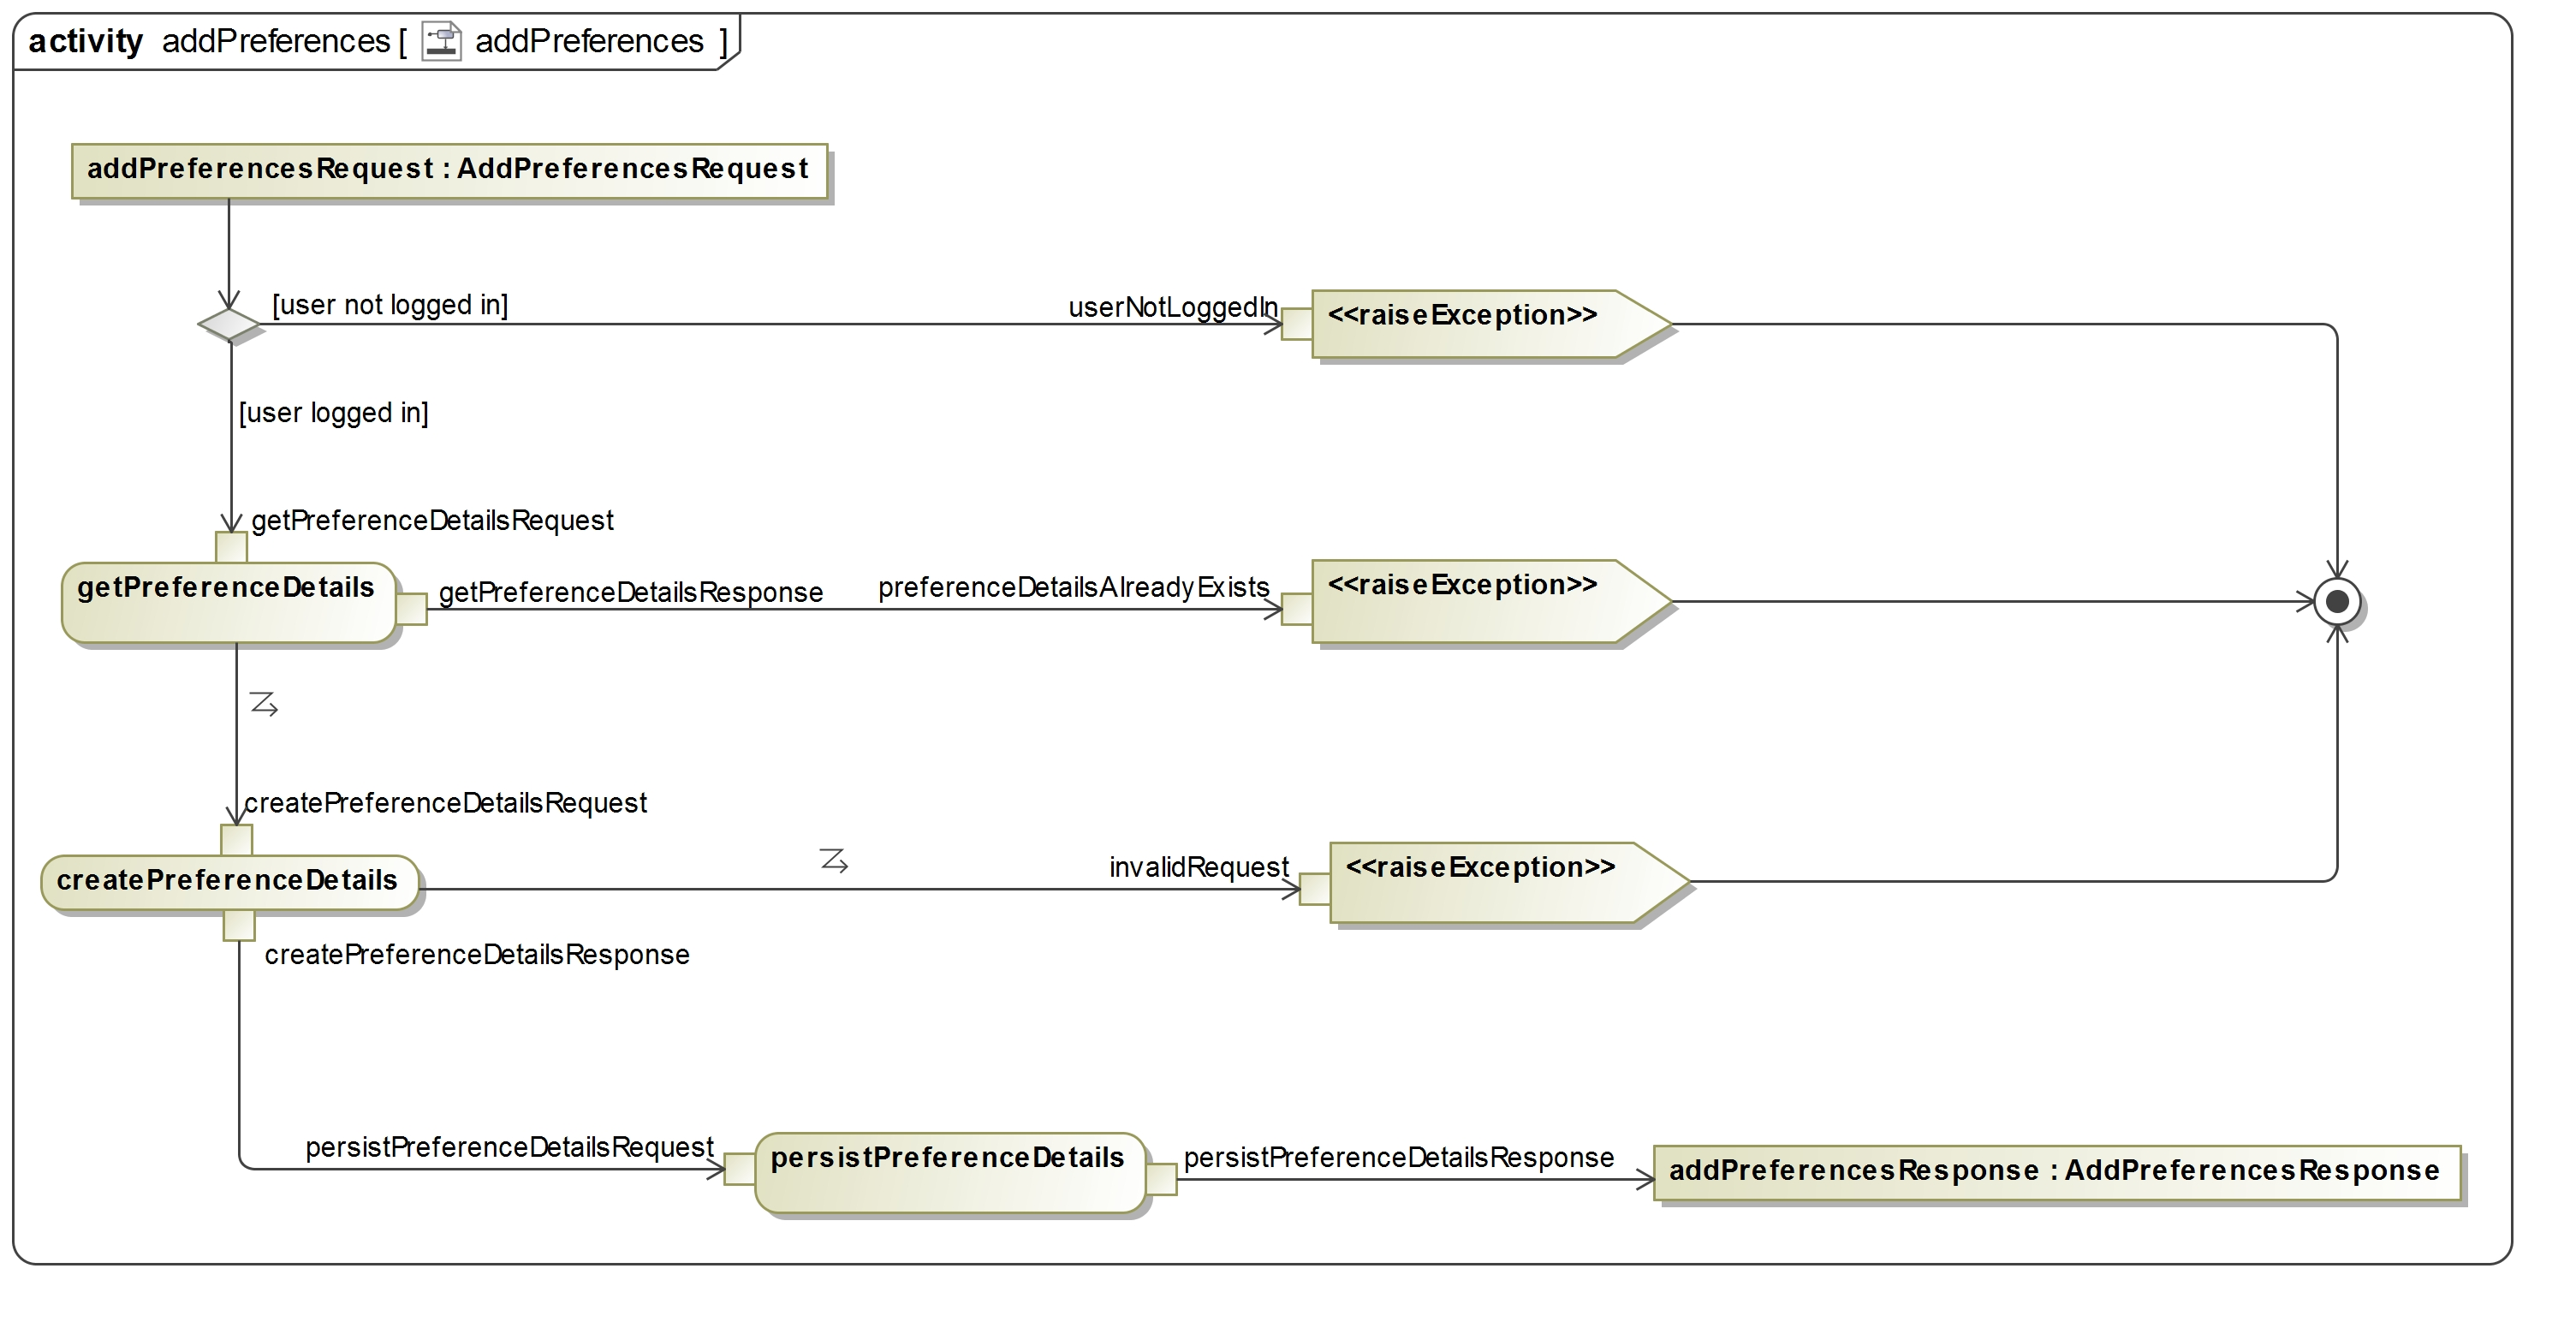
\includegraphics[scale=0.16]{../images/funcReq/addPreferencesActivityDiagram.jpg}
	\caption{The activity diagram for addPreferences \label{overflow}}
\end{figure}

\subsubsection{editPreferences}

A user, given that they are logged into the system, is able to edit any of their weather and/or disaster data preferences as long as the preference details to update exist and that the preference details when updated are not like any of the ones that already exist for the user. Below are the service contract, activity diagram and functional requirements diagram for editPreferences.

\begin{figure}[H]
	\centering
	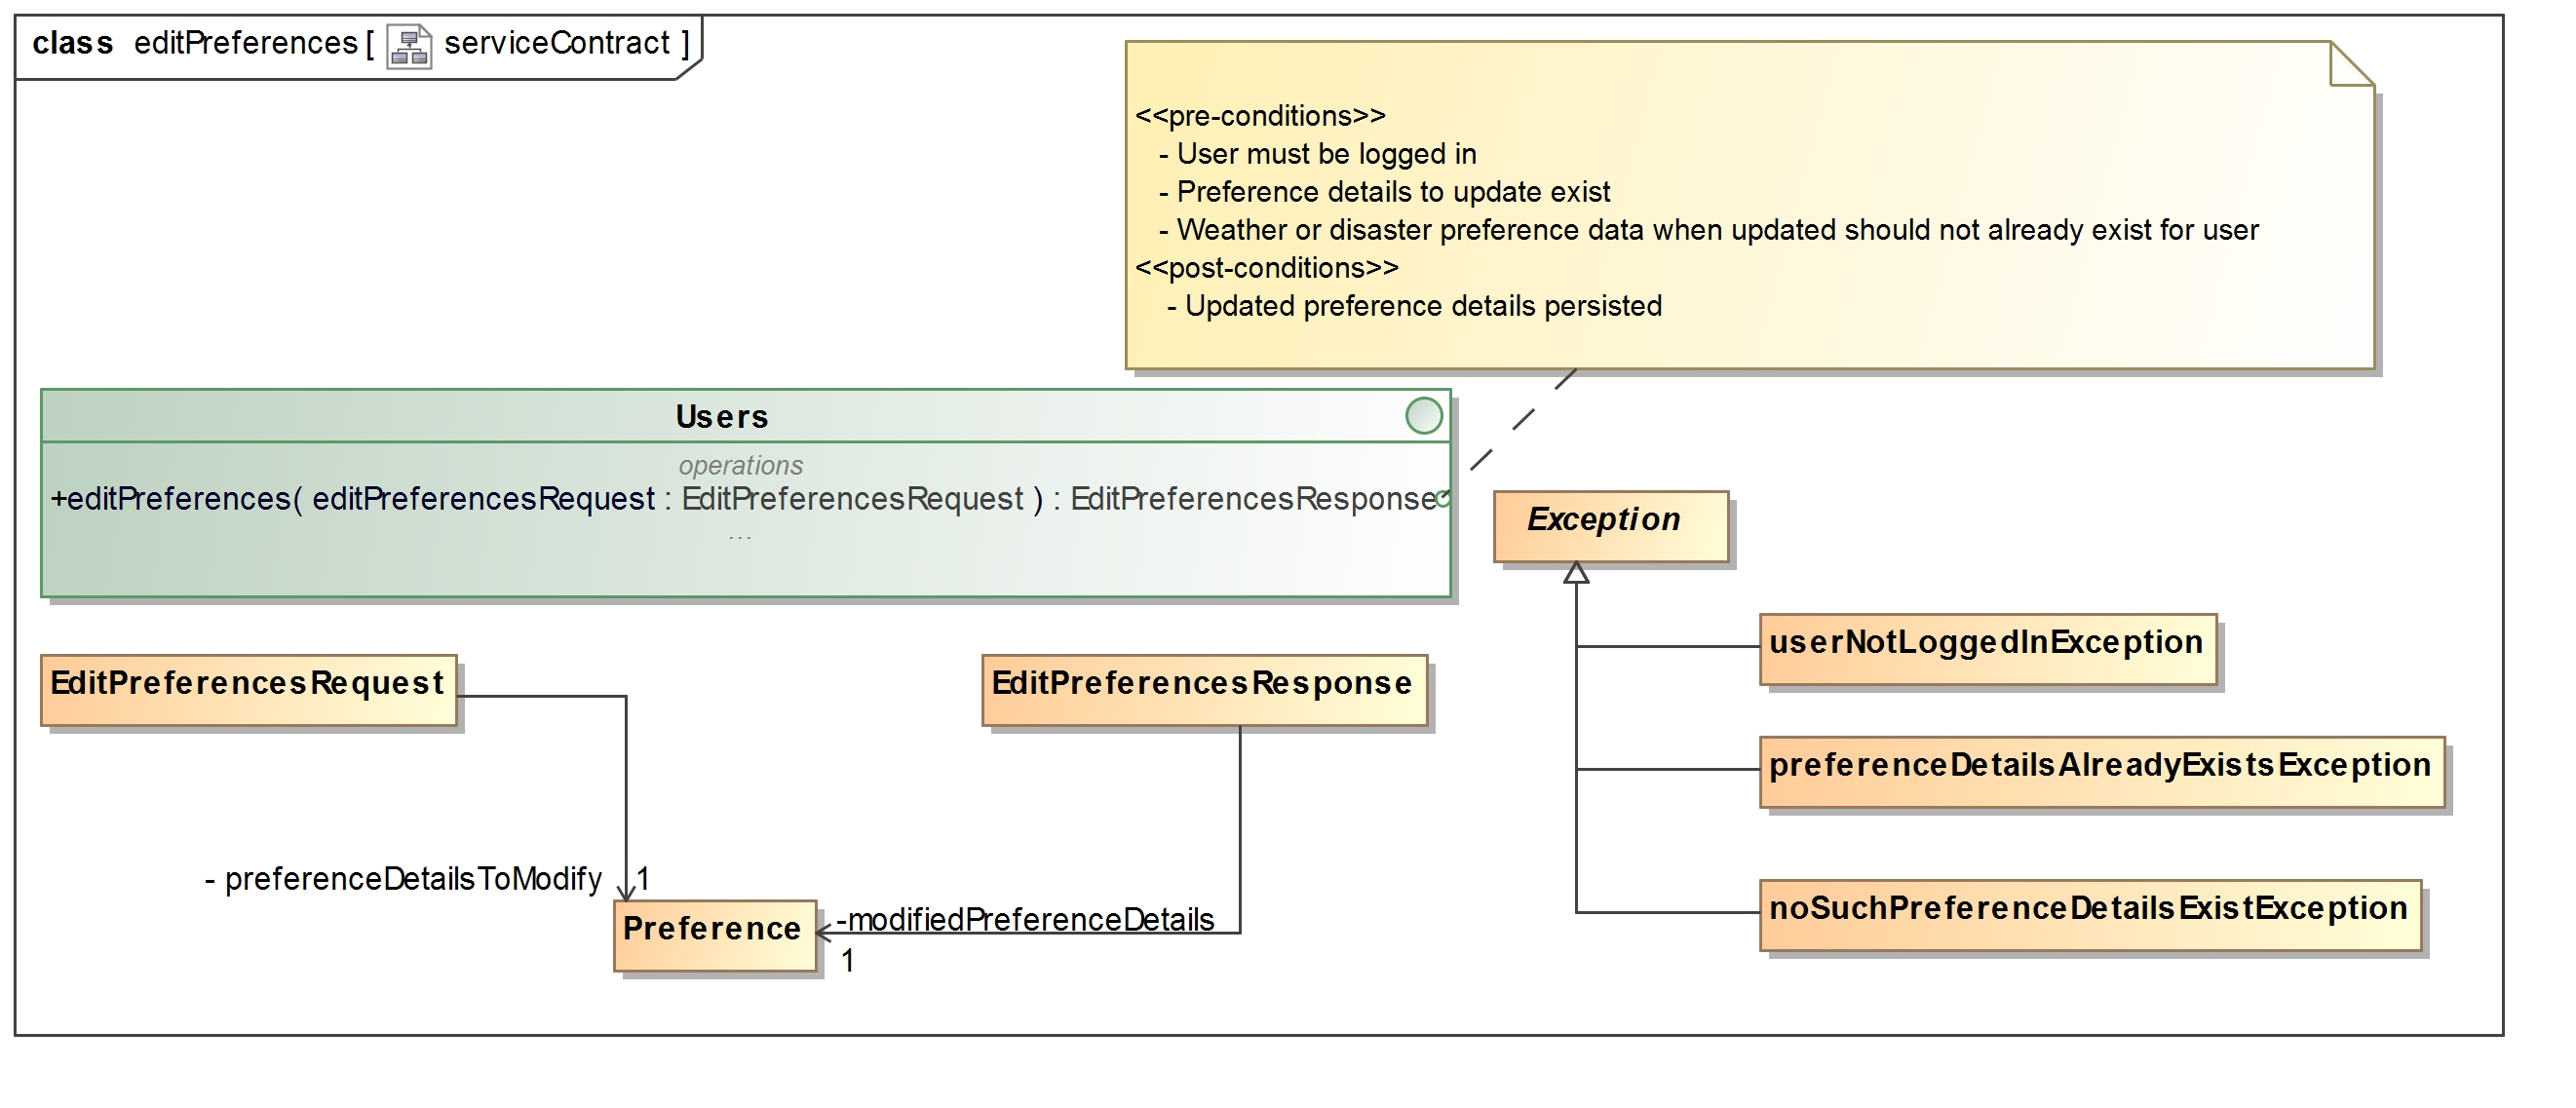
\includegraphics[scale=0.19]{../images/funcReq/editPreferencesServiceContract.jpg}
	\caption{The service contract for editPreferences \label{overflow}}
\end{figure}

\begin{figure}[H]
	\centering
	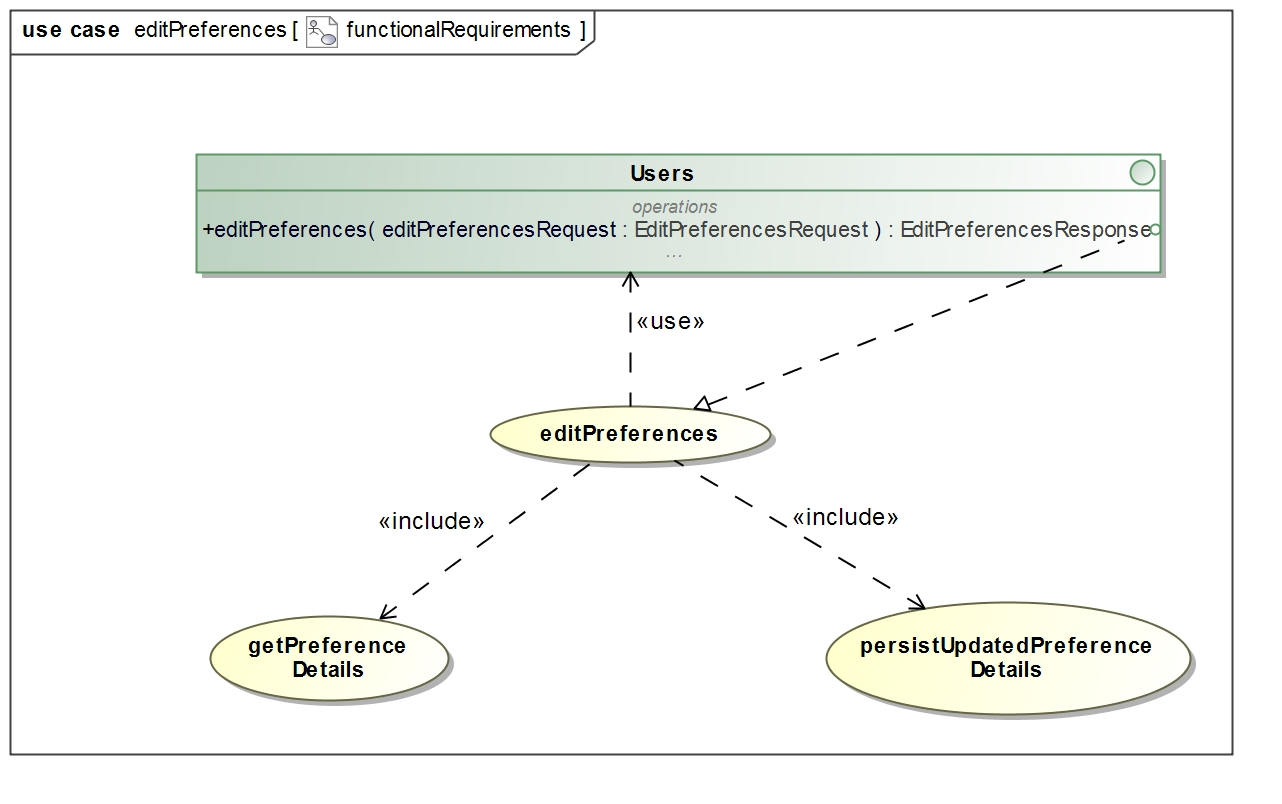
\includegraphics[width=1.1\textwidth]{../images/funcReq/editPreferencesFunctionalRequirements.jpg}
	\caption{The functional requirements diagram for editPreferences \label{overflow}}
\end{figure}

\begin{figure}[H]
	\centering
	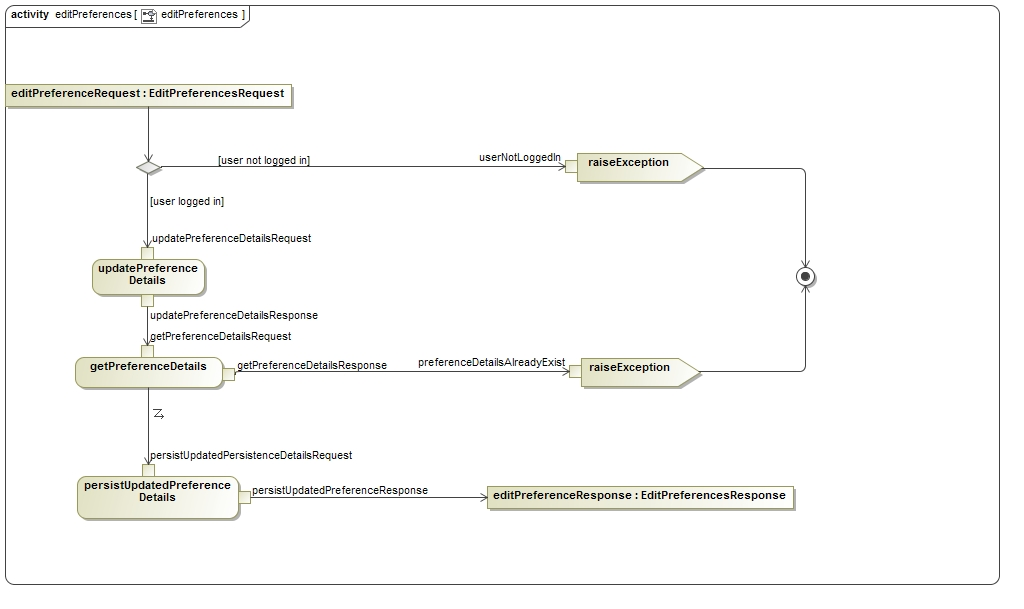
\includegraphics[scale=0.21]{../images/funcReq/editPreferencesActivityDiagram.jpg}
	\caption{The activity diagram for editPreferences \label{overflow}}
\end{figure}

\subsubsection{viewPreferences}

A user, given that they are logged into the system, is able to view any of their weather and/or disaster preferences as long as they have already added those preferences. Below are the service contract, activity diagram and functional requirements diagram for viewPreferences.

\begin{figure}[H]
	\centering
	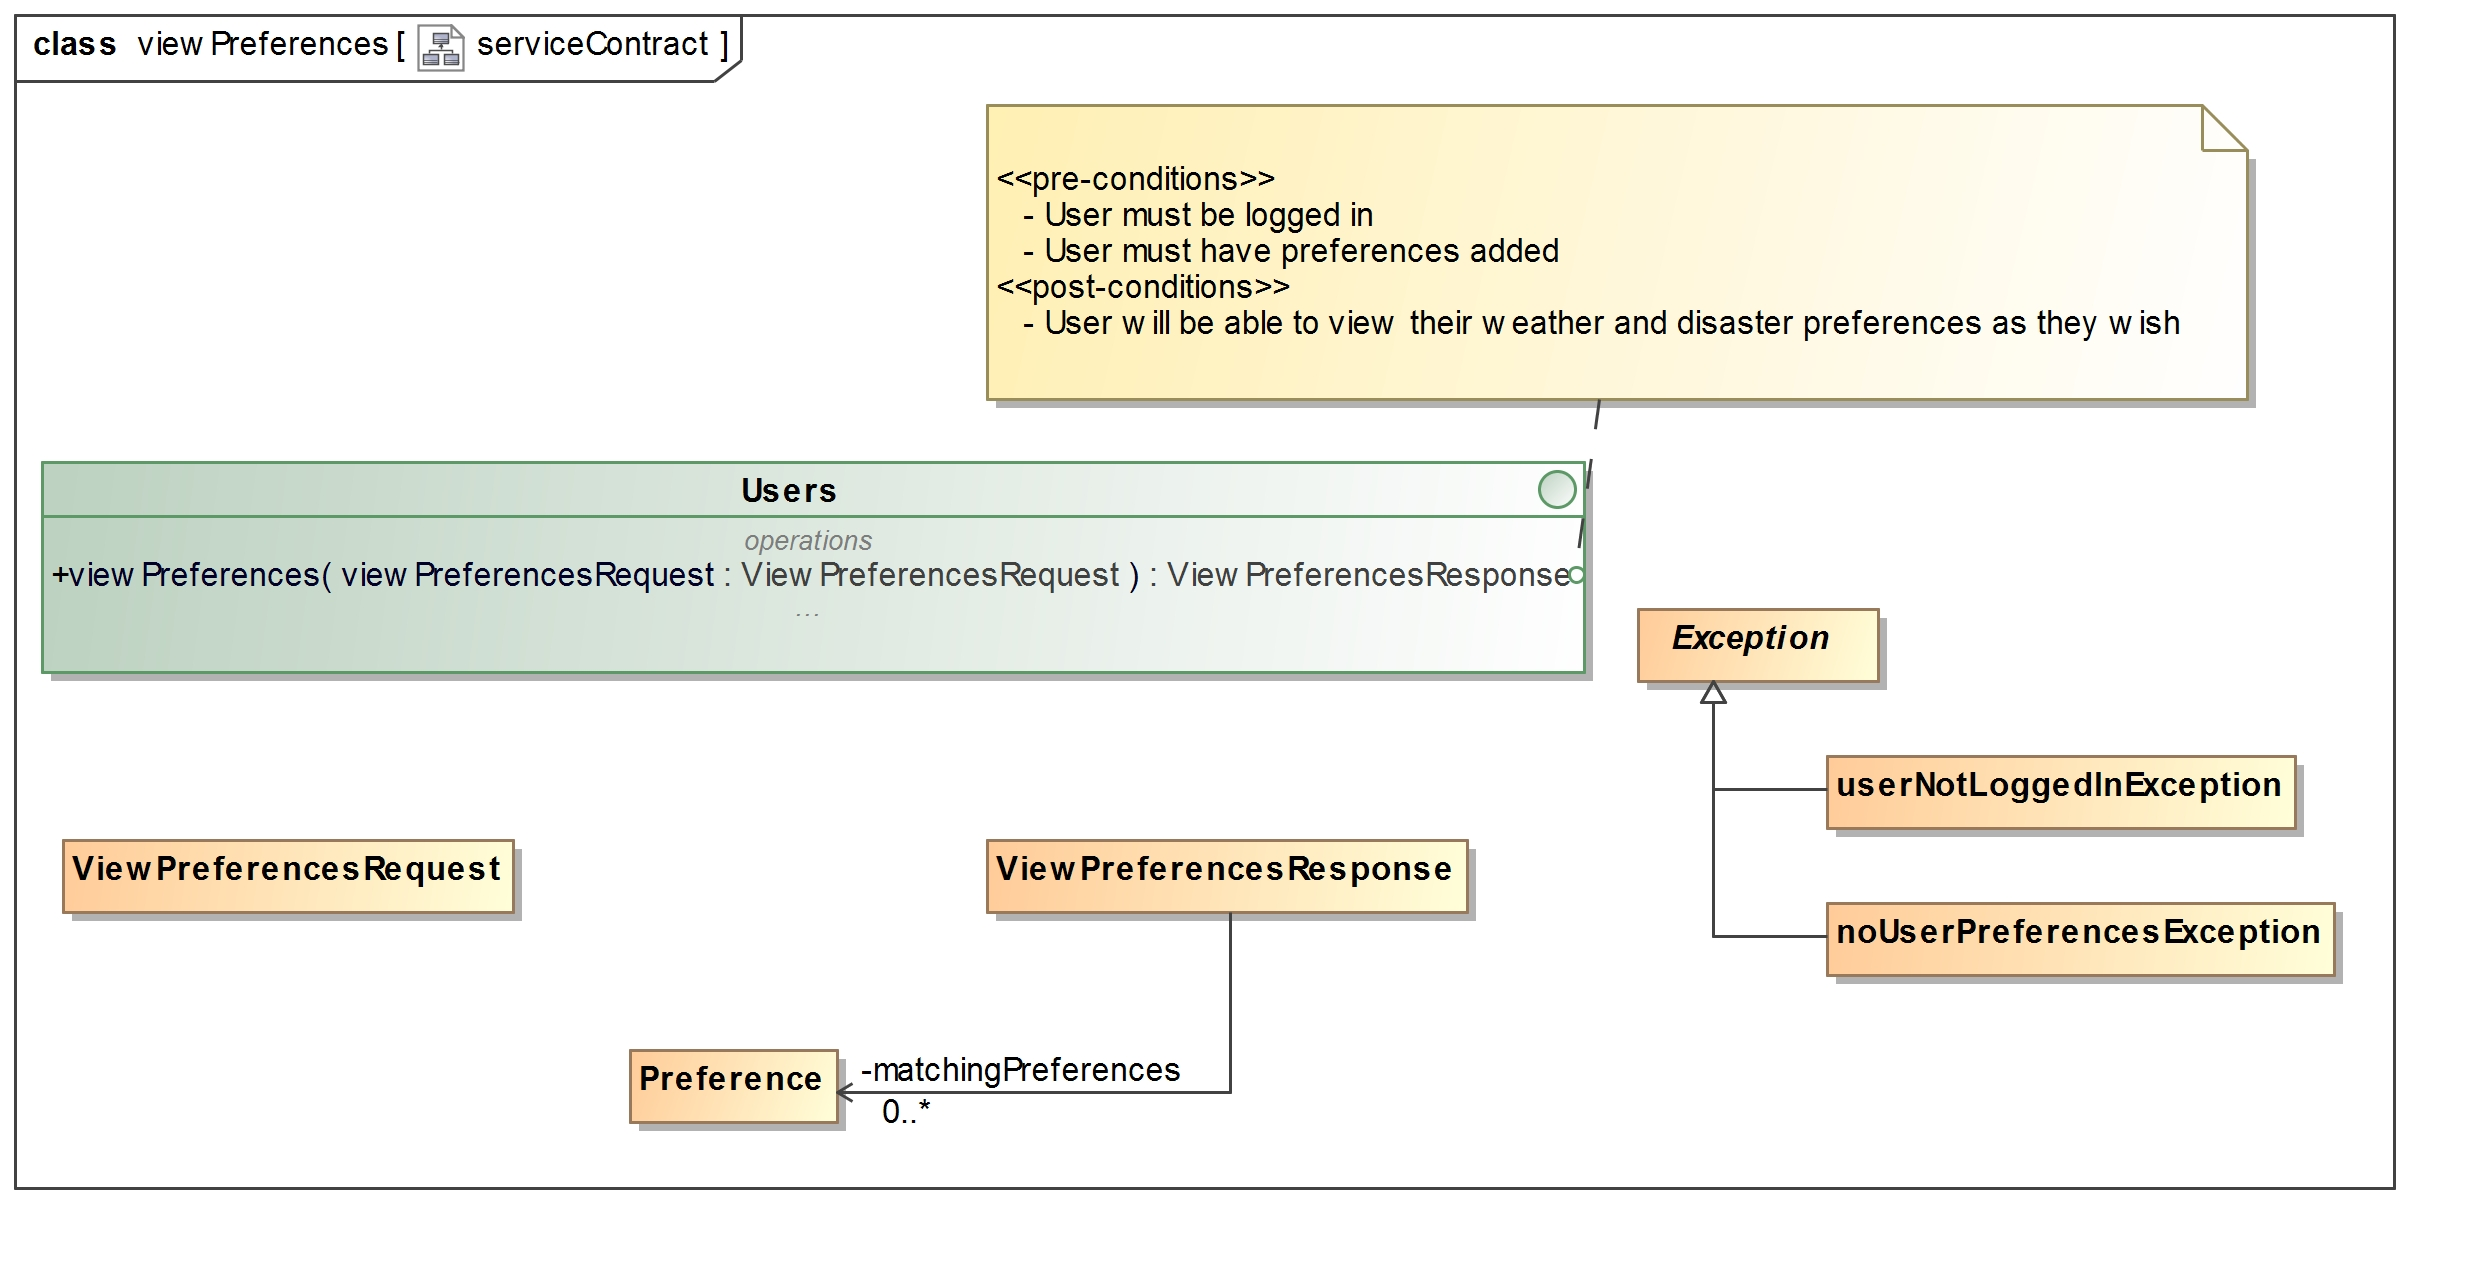
\includegraphics[scale=0.2]{../images/funcReq/viewPreferencesServiceContract.jpg}
	\caption{The service contract for viewPreferences \label{overflow}}
\end{figure}

\begin{figure}[H]
	\centering
	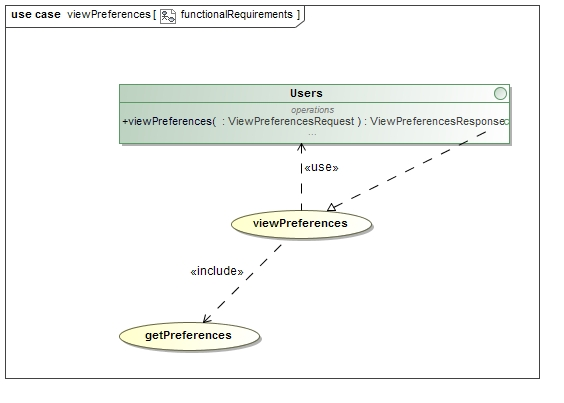
\includegraphics[width=1.1\textwidth]{../images/funcReq/viewPreferencesFunctionalRequirements.jpg}
	\caption{The functional requirements diagram for viewPreferences \label{overflow}}
\end{figure}

\begin{figure}[H]
	\centering
	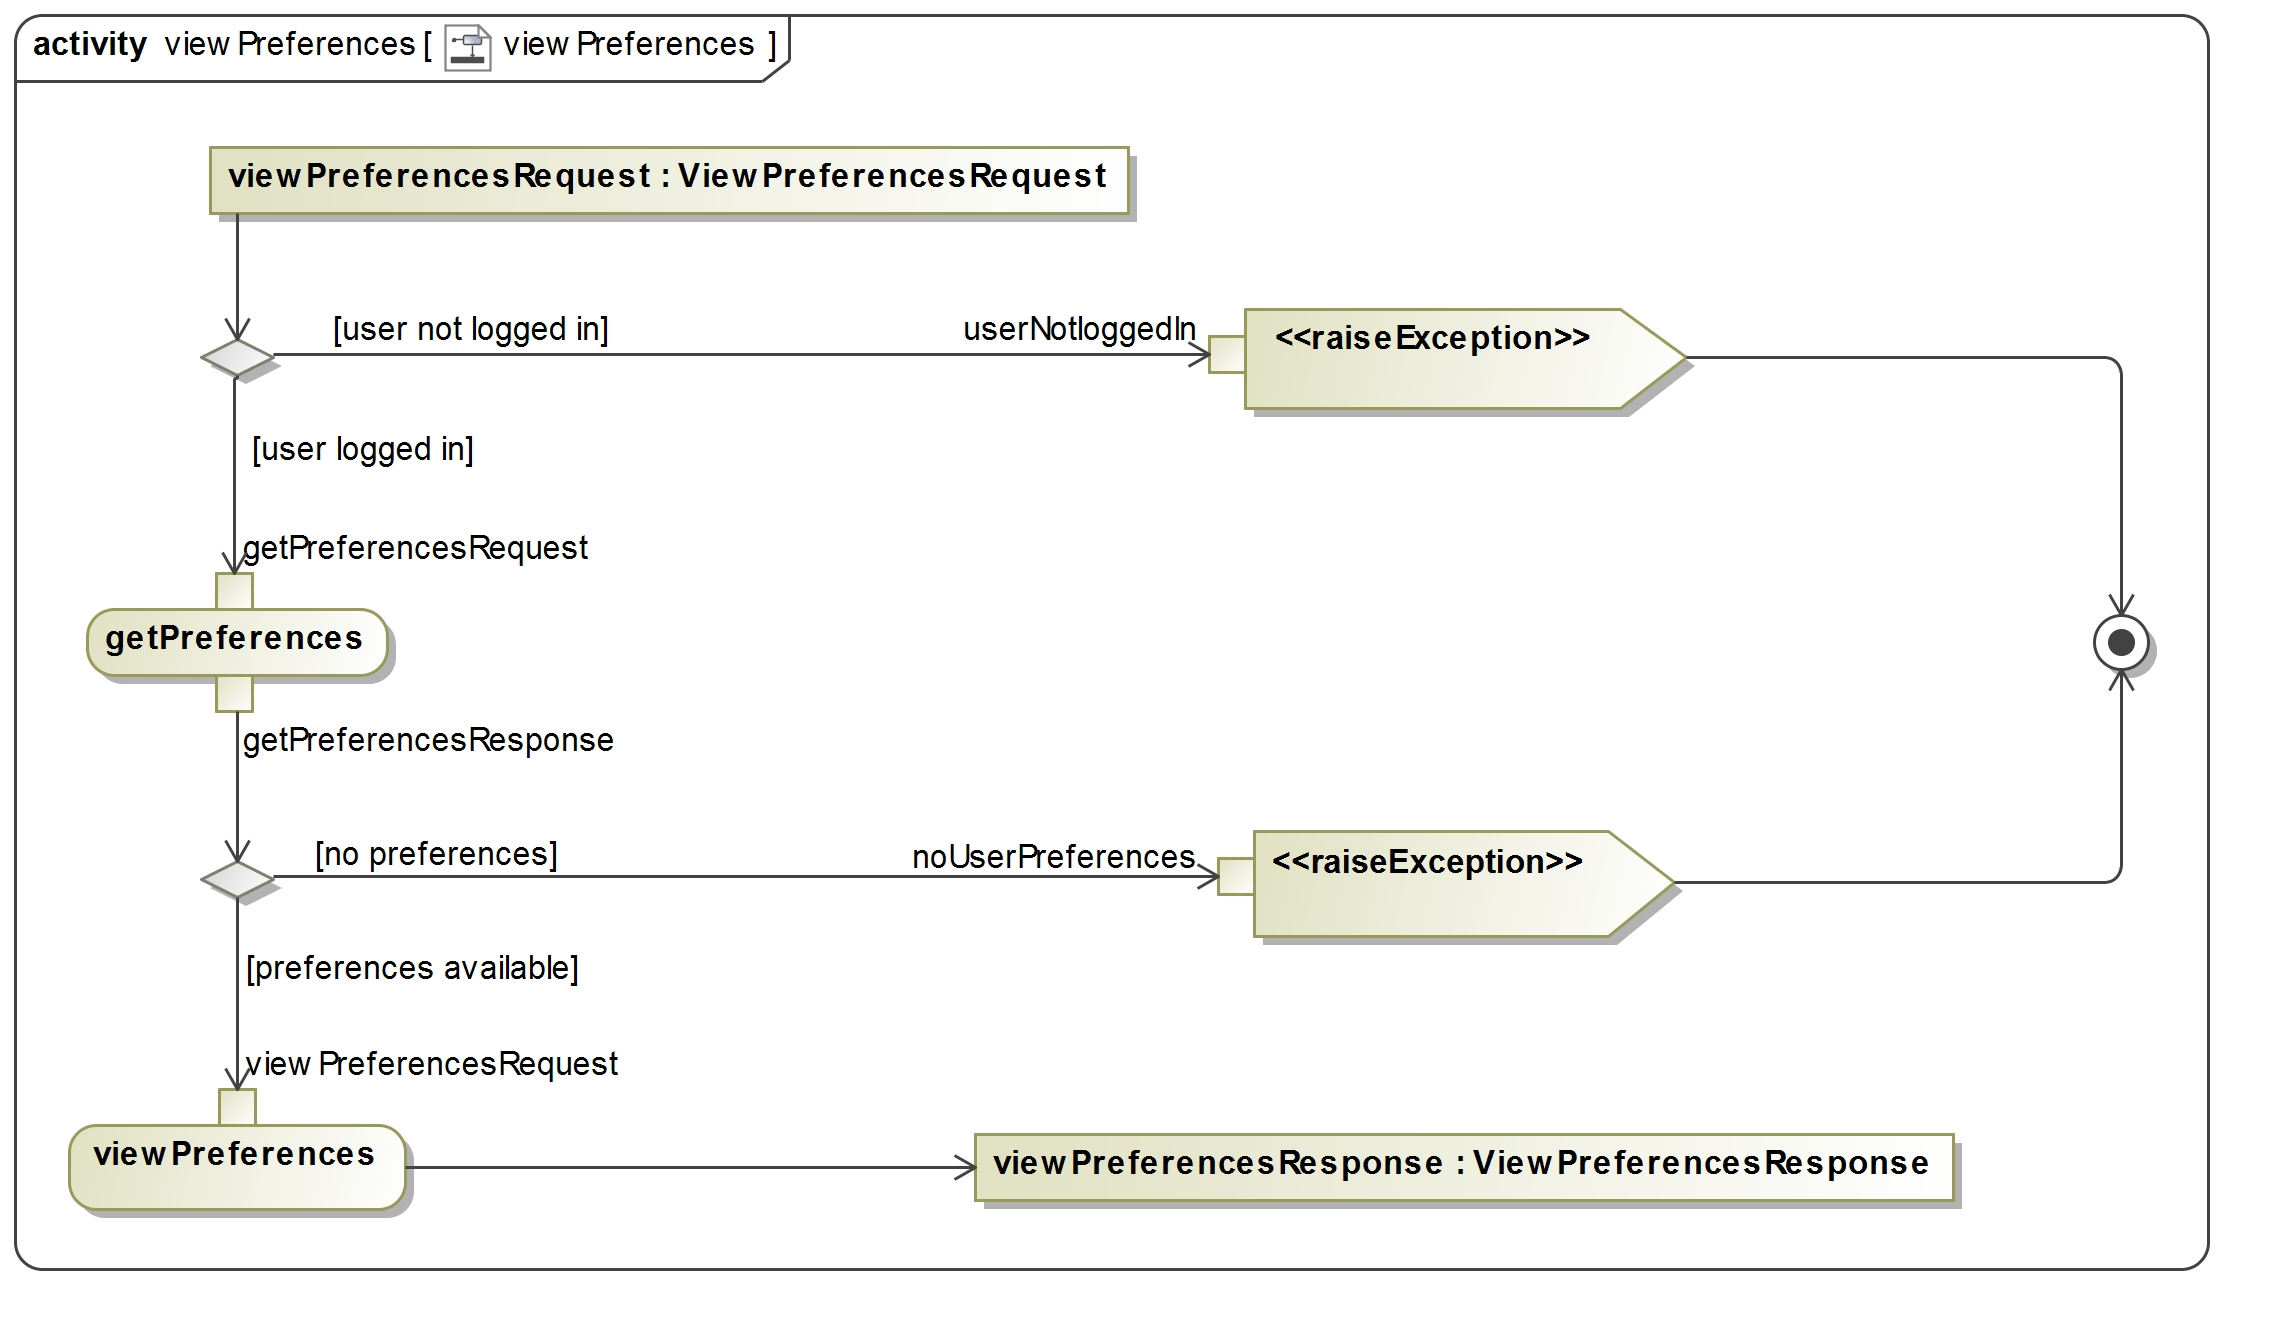
\includegraphics[scale=0.22]{../images/funcReq/viewPreferencesActivityDiagram.jpg}
	\caption{The activity diagram for viewPreferences \label{overflow}}
\end{figure}